% Online Appendix. Sections S1 to S3 give the details of the allocation, the controller and the synthetic market;
% S4 holds the supplementary results. Supplementary tables and figures sit with the section that uses them.

% appendix_a.tex
% Online Appendix: allocation details (closed forms, cone programs, hedge stage, benchmarks, bandit, parameters).
% Agent A draft, 2026-10-30. Sources: code/src/Allocators.jl, AllocatorsLongShort.jl, AllocatorsMeanVariance.jl,
% code/src/Screens.jl, code/src/StudyBacktest.jl, config/study.toml, results/calibration_summary.toml,
% code/test/test_allocators_utility.jl. The source of each number is in a comment on the line above it.

\section{Allocation details}\label{app:allocation}

\paragraph{Closed forms under the budget alone.}
We derive the optima of Table~\ref{tab:utilities} for a decision without hedge names. Let $\mathcal{P}$ be the names
with $\gamma_i > 0$ and $F = W - \sum_{j \notin \mathcal{P}} \varepsilon S_j$ (USD) the wealth left after the floors
of the other names. Each utility increases in every $n_i$ with $i \in \mathcal{P}$, so the budget
$\sum_{i \in \mathcal{P}} S_i n_i \le F$ binds. For CD, stationarity of the Lagrangian gives
$\gamma_i / n_i = \nu S_i$ with multiplier $\nu > 0$ (USD$^{-1}$), so $S_i n_i = \gamma_i / \nu$, and the budget sets
$\nu = \sum_{j \in \mathcal{P}} \gamma_j / F$, hence $w_i = (F/W)\, \gamma_i / \sum_{j \in \mathcal{P}} \gamma_j$.
For CES with $0 < \rho < 1$ ($\eta > 1$) the rule maximizes the concave sum $\sum \gamma_i n_i^{\rho}$; with
$\rho < 0$ ($0 < \eta < 1$) the outer power $1/\rho$ is negative, so the rule minimizes the convex sum
$\sum \gamma_i n_i^{\rho}$. In both cases stationarity gives $\rho\, \gamma_i\, n_i^{\rho - 1} = \nu S_i$ with $\nu$
of the sign of $\rho$, and because $1/(\rho - 1) = -\eta$,
\begin{equation}
n_i = C \left( \frac{\gamma_i}{S_i} \right)^{\eta}, \qquad
C = \frac{F}{\sum_{j \in \mathcal{P}} S_j (\gamma_j / S_j)^{\eta}}, \qquad
w_i = \frac{F}{W}\, \frac{\gamma_i^{\eta} S_i^{1-\eta}}{\sum_{j \in \mathcal{P}} \gamma_j^{\eta} S_j^{1-\eta}}.
\label{eq:S-ces-closed}
\end{equation}
As $\eta \to 0$ every name in $\mathcal{P}$ receives the same share count, a price-weighted book; as
$\eta \to \infty$ the budget goes to the name with the largest $\gamma_i / S_i$. The same steps with $w_i$ in place of
$n_i$ and the budget $\sum_{i \in \mathcal{P}} w_i \le F/W$ give CESw,
$w_i = (F/W)\, \gamma_i^{\eta} / \sum_{j \in \mathcal{P}} \gamma_j^{\eta}$, which tends to equal weights as
$\eta \to 0$ and to the name with the largest $\gamma_i$ as $\eta \to \infty$. For SG every name of $\mathcal{N}$ holds
$n_i \ge b_i$ and the names outside $\mathcal{P}$ hold exactly $b_i$. Writing $e_i = n_i - b_i$ for the excess shares,
SG maximizes $\sum_{i \in \mathcal{P}} \gamma_i \ln e_i$ subject to
% config/study.toml sg_baseline = 0.01
$\sum_{i \in \mathcal{P}} S_i e_i \le W - \sum_{j \in \mathcal{N}} S_j b_j = W (1 - 0.01\,\lvert\mathcal{N}\rvert)$,
which is the CD problem on the excess shares, so
\begin{equation}
w_i = 0.01 + \left( 1 - 0.01\,\lvert\mathcal{N}\rvert \right) \frac{\gamma_i}{\sum_{j \in \mathcal{P}} \gamma_j},
\qquad i \in \mathcal{P}.
\label{eq:S-sg-closed}
\end{equation}
A feasible SG book therefore needs $\lvert\mathcal{N}\rvert \le 100$, and a positive excess needs
$\lvert\mathcal{N}\rvert < 100$. The unit tests checked Eq.~\ref{eq:S-sg-closed} against the solver on a three-name
% code/test/test_allocators_utility.jl: rtol = 1e-4 (Clarabel stops at ALMOST_OPTIMAL there)
problem to a relative tolerance of $10^{-4}$, and on the hand-picked list the CD, CES and CESw solver weights stayed
% results/limits_day.csv: max |weight - closed_form| = 1.03e-5
within $1.0 \times 10^{-5}$ of their closed forms.

\paragraph{Cone programs.}
We use the cone conventions of MathOptInterface. The exponential cone is the closure of
$\{(x, y, z) : y > 0,\ y\, e^{x/y} \le z\}$, so, with an auxiliary variable $t_i$ per name, $(t_i, 1, n_i)$ in the
cone is $t_i \le \ln n_i$. CD maximizes
% Allocators.jl allocate(::MyCobbDouglasRule): lower bound 1e-8 on preferred shares
$\sum_{i \in \mathcal{P}} \gamma_i t_i$ with $n_i \ge 10^{-8}$, and SG puts $(t_i, 1, n_i - b_i)$ in the cone. The
power cone with exponent $a \in (0, 1)$ is $\{(x, y, z) : x^{a} y^{1-a} \ge \lvert z \rvert,\ x, y \ge 0\}$. The CES
rules act on a scaled variable $u_i = n_i \sum_{j \in \mathcal{P}} S_j / W$ (CES), which equals one at equal share
counts that spend $W$, or $u_i = \lvert\mathcal{P}\rvert\, w_i$ (CESw), which equals one at equal weights; a common
positive scale multiplies $\sum \gamma_i u_i^{\rho}$ by a constant and leaves the optimum unchanged, and it keeps
$u_i$ near one at any wealth and basket size. For $\eta > 1$ the program puts $(u_i, 1, t_i)$ in the power cone with
exponent $\rho$, so $t_i \le u_i^{\rho}$, and maximizes $\sum \gamma_i t_i$. For $\eta < 1$ it puts $(t_i, u_i, 1)$ in
the power cone with exponent $\eta$, so $t_i^{\eta} u_i^{1-\eta} \ge 1$, which is $t_i \ge u_i^{\rho}$, and minimizes
$\sum \gamma_i t_i$. At $\eta = 1$ both CES rules call CD. The volatility cap puts
$(\sigma_{\mathrm{SPY}}, L^{\top} w)$ in the second-order cone. The turnover budget uses slack variables
$v_i \ge \lvert n_i - n_i^{\mathrm{prev}} \rvert$ with $\bar c\, \bar S \sum_i v_i \le B$, added only when the largest
possible share change could break the budget. A name held at its floor enters the limits as a constant, and a limit
row made only of constants is checked directly instead of being sent to the solver, because all-zero rows degraded
% Allocators.jl _add_le!: CD with one floor, share error 1.3e-5 with zero rows, 2e-6 without
Clarabel's accuracy (a share error of $1.3 \times 10^{-5}$ with them against $2 \times 10^{-6}$ without, on a CD
test). LS uses two exponential-cone blocks, $(t_i^{+}, 1, n_i^{+})$ for the long names with $\gamma_i > 0$ and
% AllocatorsLongShort.jl: lower bound 1e-8 on n+ and n-
$(t_i^{-}, 1, n_i^{-})$ for the short names, with $n_i^{\pm} \ge 10^{-8}$, and applies the limits to the signed
% Allocators.jl _CLARABEL_ATTRIBUTES and the comment above them
weights $w_i = (n_i^{+} - n_i^{-}) S_i / W$. We set Clarabel's duality-gap tolerances to $10^{-12}$ because the
utility is flat at its optimum, so the share error scales with the square root of the gap: on a three-name CD test the
solver's shares missed the closed form by $2.5 \times 10^{-5}$ at a gap tolerance of $10^{-9}$ and by
$6 \times 10^{-9}$ at $10^{-12}$. An exception thrown inside a solver, such as the domain error that Clarabel
$0.11.1$ raised in its power-cone barrier for some CES problems at $\eta \le 0.25$ and $\eta \ge 4$, counted as that
solver not accepting the problem, and the decision moved on to SCS.

\paragraph{The hedge stage.}
Let $\mathcal{H}_f$ be the free hedge names, the pool names with $\gamma_i \le 0$, and $n^{(1)}$ the first-stage
shares. The second stage holds every name with a utility term at $n_i^{(1)}$ as a fixed variable, so its share
change still counts toward the turnover budget, holds every other name outside $\mathcal{H}_f$ at its floor, and
solves
\begin{equation}
\min_{n_i \ge f_i,\ i \in \mathcal{H}_f} \ \sum_{i \in \mathcal{H}_f} w_i
\quad \text{subject to the limits of Eq.~\ref{eq:allocation} (and the 130/30 rows for LS)},
\label{eq:S-hedge}
\end{equation}
% Allocators.jl _min_hedge, _solve_utility; _HEDGE_TIEBREAK = 1e-6
with $f_i$ the floor of hedge name $i$ ($\varepsilon$ for CD, CES and CESw, $b_i$ for SG and $10^{-8}$ for LS). The
first stage already subtracts $10^{-6} \sum_{i \in \mathcal{H}_f} w_i$ from the utility, but that cost is below the
solver's dual accuracy and alone would leave hedge holdings of several percent of wealth along the flat direction;
Eq.~\ref{eq:S-hedge} removes them. For SG with no positive score and a finite $\beta$ cap, the second stage runs
with no fixed names and finds the least hedge holding that lets the baselines meet every limit.

\paragraph{Minimum variance and tangency.}
Both benchmarks use long-only shares with no floors and the expected growth rates
$\mu_{g,i} = \alpha_i + \beta_i \tilde g_M$. They first solve
$s = \min\big(1, \max \sum_i w_i\big)$ over the budget, single-name, $\beta$ and turnover limits without the
volatility cap. MinVar then minimizes $w^{\top} \Sigma_g w$ over the same limits with
% AllocatorsMeanVariance.jl _S_TOL = 1e-7
$\sum_i w_i \ge s - 10^{-7}$. Tangent, with excess growth $e = \mu_g - g_f \mathbf{1}$, first finds the best feasible
excess growth $\bar e = \max e^{\top} w$ over that set; when $\bar e \le 10^{-6}\, s \max_i \lvert e_i \rvert$ no
% AllocatorsMeanVariance.jl _MIN_EXCESS_REL = 1e-6
feasible mix has positive excess growth and the rule falls back to the MinVar portfolio. Otherwise it applies the
Charnes--Cooper change of variables~\cite{charnes1962} $y = \kappa n$, $v = \kappa w$ with $\kappa \ge 0$, and solves
\begin{equation}
\min_{y \ge 0,\ \kappa \ge 0} \ v^{\top} \Sigma_g\, v
\quad \text{subject to} \quad e^{\top} v = \bar e, \qquad \textstyle\sum_i v_i \ge (s - 10^{-7})\,\kappa,
\label{eq:S-tangent}
\end{equation}
with the right-hand side of every limit multiplied by $\kappa$, and sets $w_{\mathrm{mix}} = v / \kappa$. Fixing
$e^{\top} v$ at $\bar e$ instead of one leaves the optimum unchanged, because the Sharpe ratio does not depend on the
scale of $w$, and it keeps $\kappa = \bar e / e^{\top} w_{\mathrm{mix}} \ge 1$, so the division does not amplify solver
error. Each mix is then scaled by $c = \min\big(1, \sigma_{\mathrm{SPY}} / \sqrt{w_{\mathrm{mix}}^{\top} \Sigma_g\,
w_{\mathrm{mix}}}\big)$ with the rest in cash. Scaling down keeps the budget, the single-name caps and the $\beta$ cap,
whose bound is never negative; the turnover budget is checked again, and a scaled book that breaks it keeps the
previous holdings. An earlier version forced $\sum_i w_i$ to the largest investment the volatility cap allowed, which
left a single feasible portfolio whenever the cap bound, so MinVar and Tangent coincided; the two-fund form, a risky
mix scaled against cash~\cite{tobin1958}, avoids this.

\paragraph{The bandit selection rule.}
One sector's bandit at a pick on day $t$ runs as in Algorithm~\ref{alg:S-bandit}. The window starts $d$ run over
$\mathcal{D}_t = \{t - 272, \dots, t - 21\}$, the $252$ starts whose 21-day windows end on days $t - 251$ through $t$.
% Bandit.jl _stream_seed: (seed * 1,000,003 + date value) * 64 + sector rank
The random stream of the sector with rank $r$ (sectors in alphabetical order) is seeded with
$(\text{seed} \cdot 1{,}000{,}003 + \text{date}) \cdot 64 + r$, where date is the day count of the pick date, so a
pick depends only on the run seed, the date and the sector.

\begin{algorithm}[tp]
\caption{Bandit selection rule for one sector at a pick on day $t$.}
\label{alg:S-bandit}
\begin{algorithmic}[1]
  \REQUIRE The sector's names $j = 1, \dots, A$; excess growth rates $x_j(d)$ (yr$^{-1}$) for window starts
    $d \in \mathcal{D}_t$; a random stream seeded by the run seed, the date and the sector.
  \ENSURE The $3$ names with the highest mean reward.
  \IF{$A \le 3$}
    \RETURN all $A$ names
  \ENDIF
  \STATE $M \gets \min(\max(50A, 500), 5000)$; $\hat\mu_j \gets 0$ and $c_j \gets 0$ for every $j$; draw a random
    permutation $\pi$ of $1, \dots, A$ as the tie-break rank
  \FOR{$k = 1, \dots, M$}
    \STATE $\epsilon_k \gets 1$ if $k = 1$, else $\max\{0.05,\, \min[1,\, k^{-1/3} (A \ln k)^{1/3}]\}$
    \IF{$\mathrm{Uniform}(0,1) < \epsilon_k$ or no arm has been pulled}
      \STATE $a \gets$ an arm drawn uniformly from $1, \dots, A$ \hfill \COMMENT{explore}
    \ELSE
      \STATE $a \gets \arg\max_{j : c_j > 0} \hat\mu_j$, ties to the smallest $\pi_j$ \hfill \COMMENT{exploit}
    \ENDIF
    \STATE $d \gets$ a start drawn uniformly from $\mathcal{D}_t$; $c_a \gets c_a + 1$;
      $\hat\mu_a \gets \hat\mu_a + (x_a(d) - \hat\mu_a)/c_a$
  \ENDFOR
  \RETURN the first $3$ names ordered by: pulled before unpulled, then $\hat\mu_j$ descending, then $\pi_j$ ascending
\end{algorithmic}
\end{algorithm}

\paragraph{Parameters.}
The settings of the allocation, the score and the selection rules, with the calibrated values from 2014--2024, are
in Table~\ref{tab:S-allocation-params}.

\clearpage
% Table S: settings of the allocation, the score and the selection rules.
% Sources: config/study.toml (every setting; section in brackets), results/calibration_summary.toml (calibrated
% values G, sigma_m, vol_cap_annual, m_m, v_m, lambda), code/Manifest.toml (package versions),
% code/src/Allocators.jl (_CLARABEL_ATTRIBUTES, _HEDGE_TIEBREAK), code/src/Backtest.jl (_BT_eps, _BT_HELD_W).
\begin{table}[H]
\centering
\footnotesize
\setlength{\tabcolsep}{4pt}
\caption{\textbf{Settings of the allocation, the score and the selection rules.} Windows and spans are in trading
days. Calibrated values were fitted once on 2014-01-03 to 2024-12-31 and then held fixed.}
\label{tab:S-allocation-params}
\begin{tabular}{@{}lll@{}}
\toprule
Setting & Symbol & Value \\
\midrule
% config/study.toml [sim], [market]; results/calibration_summary.toml
\multicolumn{3}{@{}l}{\emph{Score}} \\
Half-life of the weighted least-squares fit & $h$ ($\delta = 2^{-1/h}$) & $63$ days \\
Prior weight of the 2014--2024 fit & $N_0$ & $63$ observations \\
SPY growth mean; variance (prior, calibrated) & & $0.106$~yr$^{-1}$; $7.51$~yr$^{-2}$ \\
market growth average, EMA span & $\tilde g_M$ & $252$ days \\
market state, EMA spans & $\xi$ & $21$ and $63$ days \\
market state gain (calibrated, $99\%$ rule) & $G$ & $21.23$ \\
floor on $\lvert\beta_i\rvert$ in the score & & $0.1$ \\
\addlinespace
% config/study.toml [limits], [costs], [covariance]; results/calibration_summary.toml
\multicolumn{3}{@{}l}{\emph{Limits}} \\
single-name cap: picks; other names & $\bar w_i$ & $\max(0.10, 1.5/K)$; $0.10$ \\
volatility cap (calibrated) & $\sigma_{\mathrm{SPY}}$ & $2.741$~yr$^{-1}$ ($17.3\%$ annualized) \\
residual covariance window; shrinkage & & $126$ days; $0$ \\
half spread; turnover budget & $\bar c$; $B$ & $5$~bps; $0.10\,W$ \\
sector cap & & none \\
\addlinespace
% config/study.toml [hedge]
\multicolumn{3}{@{}l}{\emph{Hedge}} \\
$\beta$ cap & $\bar\beta$ & $\max(0, 1 - \xi_t)$ \\
pool size; down-day beta lookback & $H$ & $5$ names; $252$ days \\
\addlinespace
% config/study.toml [allocators]; Backtest.jl _BT_eps, _BT_HELD_W; Allocators.jl _HEDGE_TIEBREAK
\multicolumn{3}{@{}l}{\emph{Weighting}} \\
CES elasticity & $\eta$; $\rho$ & $0.5$; $-1$ \\
Stone--Geary baseline & $b_i S_i$ & $0.01\,W$ \\
floor of names with $\gamma_i \le 0$ (CD, CES, CESw) & $\varepsilon$ & $10^{-3}$ shares \\
smallest traded target & & $0.001\,W$ \\
hedge tie-break cost & & $10^{-6}$ per unit weight \\
$130/30$ long; short; net weight & & $1.30$; $0.30$; $1.00$ \\
\addlinespace
% config/study.toml [screens], [grid]
\multicolumn{3}{@{}l}{\emph{Selection}} \\
names per sector (per-sector rules) & & $3$ ($33$ in all) \\
names, universe-wide rules (main comparison) & $K$ & $13$ \\
liquid shortlist; dollar-volume window & & $100$ names; $63$ days \\
correlation limit; window & & $0.7$; $252$ days \\
bandit lookback; reward window & & $252$ days; $21$ days \\
bandit exploration floor; pulls & $\epsilon$ & $0.05$; $50A$ within $[500, 5000]$ \\
pick interval; pick at band exit & & $21$ days; yes \\
seeds & & $5660$--$5689$ \\
\addlinespace
% code/Manifest.toml; Allocators.jl _CLARABEL_ATTRIBUTES
\multicolumn{3}{@{}l}{\emph{Solvers}} \\
modeling package; solvers & & JuMP 1.32.1; Clarabel 0.11.1, SCS 2.7.0 \\
Clarabel gap; feasibility tolerance; iterations & & $10^{-12}$; $10^{-9}$; $500$ \\
\bottomrule
\end{tabular}
\end{table}



% appendix_b.tex
% Online Appendix: estimation equations behind the controller's forecast (online single-index fit, market
% volatility, residual covariance and the choice of lambda, forecast simulation) and fill details.
% Sources: code/src/SIM.jl (ewls_init, ewls_update!, ewvar_init, ewvar_update!, estimate_sim),
% code/src/OnlineSIM.jl, code/src/Covariance.jl (growth_covariance, shrinkage_loss, choose_shrinkage),
% code/src/Calibration.jl, code/src/Projection.jl (project_gbm), code/src/Backtest.jl (_bt_fill!,
% _bt_adv, _bt_projection_seed), code/src/Bandit.jl (_stream_seed), config/study.toml,
% results/calibration_summary.toml, README.md.
% The settings table is sections/tables/tableS_controller_params.tex (label tab:S-controller-params); it is
% not \input here, so the lead author can place it with the other supplementary tables.

\section{Controller and estimation details}\label{app:controller}

This appendix gives the preparation of the price data, the estimators behind the controller's forecast and the
details of the simulated fills. The settings of every real-data run are collected in
Table~\ref{tab:S-controller-params} and the experiment grids in Table~\ref{tab:S-grids}.

\subsection{Universe and price files}

% data/sp500-sectors.csv (503 rows); 418 = tickers in all three price files with a sector, counted with
% code/src/Data.jl on data/; results/calibration_summary.toml (373 names and the sector counts)
The sector snapshot lists $503$ tickers. Of the $418$ tickers that appear in all three price files with a sector,
$373$ have a positive open and close on all $3{,}187$ trading days from 2014-01-03 to 2026-09-04: $15$ in
Communication Services, $39$ in Consumer Discretionary, $31$ in Consumer Staples, $16$ in Energy, $53$ in
Financials, $44$ in Health Care, $60$ in Industrials, $50$ in Information Technology, $17$ in Materials, $22$ in Real
Estate and $26$ in Utilities. Each price file is split-adjusted by the vendor as of its own creation date, so a
split between the creation dates of two files shows as a one-day jump at their boundary.
% code/src/Data.jl (SPLIT_GATE = 0.4, SPLIT_RATIOS, SPLIT_RATIO_TOL = 0.1, SPLIT_VOLUME_TOL = 3, SPLIT_SPY_MAX = 0.05)
At each of the two boundaries we flagged a name when its overnight log price move exceeded $0.4$ in magnitude, the
move matched a standard split ratio to within a factor of $e^{0.1}$, its volume moved in the matching direction by
a factor within $3$ of that ratio, and the overnight log move of SPY was within $0.05$ in magnitude. We then divided
the earlier prices of a flagged name by the split ratio and multiplied its earlier volumes by it, which leaves the
growth rates within each file and the dollar volumes unchanged.
% README.md (Data and its limitations); results/large_k/run.log (split basis reconciled lines)
This changed seven names, ORLY (ratio $15$), NFLX ($10$), NOW ($5$) and FAST ($2$) at 2025-01-02, and KLAC ($10$),
% README.md; code/src/Data.jl (LARGE_MOVE_WARN = 0.9)
MNST ($2$) and APH ($2$) at 2026-01-02. Two one-day close moves larger than $0.9$ in log magnitude remain, IR on
2020-03-02 and NI on 2015-07-02, both inside the calibration window, and we left them as given.

\subsection{Online single-index fit}

For each name $i$ the controller updates the intercept $\alpha_i$ ($\mathrm{yr}^{-1}$) and loading $\beta_i$
(dimensionless) of the single-index model $g_i(t) = \alpha_i + \beta_i\,g_M(t) + \varepsilon_i(t)$ once per
trading day by exponentially weighted least squares. With half-life $h$ (trading days) the decay factor is
$\delta = 2^{-1/h}$, and the weighted sums are updated with the growth rates into day $t$ as
\begin{equation}
  \begin{aligned}
    S_w &\leftarrow \delta S_w + 1, &
    S_x &\leftarrow \delta S_x + g_M(t), &
    S_y &\leftarrow \delta S_y + g_i(t),\\
    S_{xx} &\leftarrow \delta S_{xx} + g_M(t)^2, &
    S_{xy} &\leftarrow \delta S_{xy} + g_i(t)\,g_M(t), & &
  \end{aligned}
  \label{eq:ewls-update}
\end{equation}
after which
\begin{equation}
  \beta_i(t) \;=\; \frac{S_w S_{xy} - S_x S_y}{S_w S_{xx} - S_x^2},
  \qquad
  \alpha_i(t) \;=\; \frac{S_y - \beta_i(t)\,S_x}{S_w},
  \label{eq:ewls-solve}
\end{equation}
with the previous estimates kept on a day when the denominator is at most $10^{-12}$ in magnitude. The sums start
from a prior worth $N_0$ pseudo-observations. Let $\alpha_i^{\mathrm{cal}}$ and $\beta_i^{\mathrm{cal}}$ be the
ordinary least-squares fit of name $i$ on SPY over the $2{,}766$ daily growth rates of the calibration window, and
let $m_M$ ($\mathrm{yr}^{-1}$) and $v_M$ ($\mathrm{yr}^{-2}$) be the mean and population variance of SPY's daily
growth rate over the same days. The prior is
\begin{equation}
  \begin{aligned}
    &S_w = N_0, \qquad S_x = N_0\,m_M, \qquad
    S_y = N_0\big(\alpha_i^{\mathrm{cal}} + \beta_i^{\mathrm{cal}} m_M\big),\\
    &S_{xx} = N_0\big(v_M + m_M^2\big), \qquad
    S_{xy} = N_0\big(\alpha_i^{\mathrm{cal}} m_M + \beta_i^{\mathrm{cal}}(v_M + m_M^2)\big),
  \end{aligned}
  \label{eq:ewls-prior}
\end{equation}
the sums that $N_0$ observations would give if SPY's growth had the calibration mean and variance and name $i$
followed its calibration fit in the mean. Before the first update Eq.~\eqref{eq:ewls-solve} gives
$\alpha_i^{\mathrm{cal}}$ and $\beta_i^{\mathrm{cal}}$ exactly, and the weight of the prior halves every $h$ days.
% config/study.toml [sim] ewls_half_life = 63.0, ewls_prior_weight = 63.0; results/calibration_summary.toml
% (m_m = 0.10610, v_m = 7.5109, sigma_m = 2.7411, vol_cap_annual = 0.17267)
We used $h = 63$ and $N_0 = 63$, with $m_M = 0.1061$~$\mathrm{yr}^{-1}$ and $v_M = 7.511$~$\mathrm{yr}^{-2}$, and
the first update used the growth into 2025-01-02. SPY's standard deviation $\sigma_M(t)$ follows the same decay,
\begin{equation}
  \begin{aligned}
    &Q_w \leftarrow \delta Q_w + 1, \qquad Q_x \leftarrow \delta Q_x + g_M(t), \qquad
    Q_{xx} \leftarrow \delta Q_{xx} + g_M(t)^2,\\
    &\sigma_M^2(t) \;=\; \frac{Q_{xx}}{Q_w} - \left(\frac{Q_x}{Q_w}\right)^2,
  \end{aligned}
  \label{eq:ewvar}
\end{equation}
from the prior $Q_w = N_0$, $Q_x = 0$ and $Q_{xx} = N_0\,\sigma_{\mathrm{SPY}}^2$, where $\sigma_{\mathrm{SPY}} = 2.741$~$\mathrm{yr}^{-1}$ is
the sample standard deviation of SPY's daily growth rate over the calibration window ($0.1727$ when multiplied by
$\sqrt{\Delta t}$ to an annual volatility, the value that also sets the volatility cap).

\subsection{Residual covariance and the choice of the shrinkage weight}

At a re-plan on day $t$ the residual matrix holds $\varepsilon_i(s) = g_i(s) - \alpha_i(t) - \beta_i(t)\,g_M(s)$
for the names of the allocation problem over the $L_\Omega$ daily growth rates that end on day $t$. We write the sample covariance of these residuals as
$\hat\Omega_\varepsilon = D R D$, with $D$ the diagonal matrix of the sample standard deviations of the residual
columns and $R$ their sample correlation matrix, and Eq.~\eqref{eq:mpc-cov} replaces $R$ by $(1-\lambda)R +
\lambda I$. A residual column with zero variance carries no correlation information and gets zero correlation with
the others. We chose $\lambda$ once, on the calibration window, by the accuracy of the residual part of
Eq.~\eqref{eq:mpc-cov} as a forecast of portfolio variance. The anchors were the last trading days of each month
% code/src/Covariance.jl (_shrinkage_anchors, shrinkage_loss: 252-day OLS, 21-day realized window, 200
% portfolios, up to 33 names, Dirichlet(1), seed 5660, grid 0:0.1:1)
with at least $252$ trading days of the window behind them and $21$ ahead. At each anchor we fitted $\alpha_i$
and $\beta_i$ by ordinary least squares on the trailing $252$ daily growth rates, because the online fit has no
warm-up period inside the calibration window, and formed $\hat\Omega_\varepsilon$ over the trailing
$L_\Omega = 126$ growth rates. We then drew $200$ portfolios per anchor, each of up to $33$ names taken in turn
from the $11$ sectors with weights $w$ drawn from a flat Dirichlet distribution. For each portfolio the realized
variance $r$ is the sample variance of $w^{\top}\varepsilon(s)$ over the $21$ days after the anchor and the
prediction is $p(\lambda) = w^{\top}\big[(1-\lambda)\hat\Omega_\varepsilon +
\lambda\,\mathrm{diag}(\hat\Omega_\varepsilon)\big]w$. The loss of $\lambda$ is the mean over portfolios and
anchors of
\begin{equation}
  \mathcal{L}(\lambda) \;=\; \frac{r}{p(\lambda)} - \ln\frac{r}{p(\lambda)} - 1,
  \label{eq:qlike}
\end{equation}
the QLIKE loss, which ranks variance forecasts consistently when the realized variance is a noisy proxy for the
true one~\cite{patton2011}. Over the grid $\lambda = 0, 0.1, \dots, 1$ we took the $\lambda$ with the smallest mean
loss, breaking ties toward the larger $\lambda$.
% README.md (lambda calibration: forecast loss 0.353 at lambda = 0, rising steadily to 0.619 at lambda = 1);
% results/calibration_summary.toml (lambda = 0.0)
The mean loss was $0.353$ at $\lambda = 0$ and rose steadily to $0.619$ at $\lambda = 1$, so the study used
$\lambda = 0$, the full sample residual covariance.

\subsection{Forecast simulation and fills}

The simulation of Eq.~\eqref{eq:mpc-gbm} draws the daily log-price increments as $\Delta t\,\mu_g +
\sqrt{\Delta t}\,L_{\Delta} z$, with $z$ a vector of independent standard normal draws and $L_{\Delta}$ the lower
Cholesky factor of
$\Delta t\,\Sigma_g + 10^{-12} I$. The diagonal term keeps the factorization defined when $\Sigma_g$ is singular
and has no other effect at the scale of the forecast. The value of a 130/30 book on each path counts its short
positions with negative shares. The forecast standard deviation uses the $N_p - 1$ denominator.
% code/src/Backtest.jl (_bt_projection_seed: seed * 1_000_003 + Dates.value(date)); code/src/Bandit.jl
% (_stream_seed: (seed * 1_000_003 + Dates.value(date)) * 64 + s)
The paths of a re-plan come from a Mersenne Twister generator seeded with $1{,}000{,}003$ times the run seed plus
the serial day number of the decision date. The picks of a random rule use the same integer for the pick date
multiplied by $64$, and each sector's bandit adds the rank of its sector to that product, so every run is
reproducible and does not depend on the thread that runs it. At a fill,
% code/src/Backtest.jl (_BT_BISECT_ITERS = 60, _BT_ADV_DAYS = 63, ADV floored at 1 share)
the common factor that scales the buys is the largest value in $[0, 1]$ that keeps cash nonnegative after the
buys and their costs, found by $60$ bisection steps, and the average daily volume $A_i$ in Eq.~\eqref{eq:cost} is
floored at one share. Names held before a re-plan that are not part of the new allocation problem are sold at the
next open.

% tableS_controller_params.tex
% Settings of the real-data runs. Sources: config/study.toml (settings), results/calibration_summary.toml
% (calibrated values), code/src/Backtest.jl (_BT_ADV_DAYS, _BT_HELD_W), trading-day counts from
% code/src/Data.jl on data/ and talk/data/market_state.csv.
\begin{table}[H]
\centering
\small
\caption{\textbf{Controller and backtest settings.} Settings of every real-data run, from the study
configuration, with the values fitted on the calibration window. Windows, horizons and intervals are in trading
days, and growth rates are in $\mathrm{yr}^{-1}$.}
\label{tab:S-controller-params}
\begin{tabular}{@{}lll@{}}
\toprule
\textbf{Setting} & \textbf{Symbol} & \textbf{Value} \\
\midrule
\multicolumn{3}{@{}l}{\textit{Windows and wealth}} \\[2pt]
% config/study.toml [window]; 2,767 and 420 trading days counted with code/src/Data.jl
Calibration window & & 2014-01-03 to 2024-12-31 ($2{,}767$ days) \\
Trading window & & 2025-01-02 to 2026-09-04 ($420$ days) \\
Length of a trading day & $\Delta t$ & $1/252$~yr \\
Initial wealth & $W_0$ & $100{,}000$~USD \\[4pt]
\multicolumn{3}{@{}l}{\textit{Estimation}} \\[2pt]
% config/study.toml [sim], [market], [covariance]; results/calibration_summary.toml
Half-life of the online single-index fit & $h$ & $63$ days \\
Prior weight of the online fit & $N_0$ & $63$ pseudo-observations \\
SPY growth mean, 2014--2024 & $m_M$ & $0.1061$~$\mathrm{yr}^{-1}$ \\
SPY growth variance, 2014--2024 & $v_M$ & $7.511$~$\mathrm{yr}^{-2}$ \\
SPY growth SD, 2014--2024 & $\sigma_{\mathrm{SPY}}$ & $2.741$~$\mathrm{yr}^{-1}$ ($0.1727$ annualized) \\
Span of SPY's average growth rate & & $252$ days \\
Residual covariance window & $L_\Omega$ & $126$ days \\
Residual shrinkage weight & $\lambda$ & $0$ (chosen from $0, 0.1, \dots, 1$) \\[4pt]
\multicolumn{3}{@{}l}{\textit{Forecast, triggers and picks}} \\[2pt]
% config/study.toml [triggers], [screens]; code/src/Backtest.jl (_BT_HELD_W = 1e-3)
Forecast horizon & $T$ & $21$ days \\
Forecast paths & $N_p$ & $1{,}000$ \\
Band half-width & $z$ & $1.96$ standard deviations \\
Drawdown limit & $D_{\max}$ & $0.08$, peak reset at each drawdown \\
Cash revisit & & $21$ days \\
Pick interval & & $21$ days, and at band exits \\
Smallest position traded & & $0.001\,W$ \\[4pt]
\multicolumn{3}{@{}l}{\textit{Costs and cash}} \\[2pt]
% config/study.toml [costs], [allocators] borrow_rate; code/src/Backtest.jl (_BT_ADV_DAYS = 63)
Half spread & $\bar c$ & $5$~bps \\
Impact coefficient & $\kappa$ & $0.001$ \\
Window of the average daily volume & & $63$ days \\
Borrow fee on short positions & $b$ & $0.0075$~$\mathrm{yr}^{-1}$ \\
Commission & & $0$ \\
Cash growth & $g_f$ & DTB3, Eq.~\eqref{eq:riskfree} \\[4pt]
\multicolumn{3}{@{}l}{\textit{Experiment grids}} \\[2pt]
% config/study.toml [grid], [screens]; results/large_k/large_k_summary.csv (K = 100, 200)
Seeds & & $5660$ to $5689$ ($30$ per cell) \\
Names per sector (per-sector rules) & & $3$ ($33$ names) \\
Basket sizes (universe-wide rules) & $K$ & $5, 8, 13, 21, 34$, and $100$, $200$ \\
\bottomrule
\end{tabular}
\end{table}

% tableS_grids.tex
% The experiment grids of the real-data backtest. Run counts are rows with status ok in each summary file
% (every row is ok): results/tier1_summary.csv 854, results/fixed_summary.csv 427,
% results/universe_summary.csv 4,438 (4,410 universe-wide + 28 hand-picked),
% results/gamma_seeds/gamma_seeds_summary.csv 4,200 (140 labels repeat tier1 and universe runs),
% results/large_k/large_k_summary.csv 1,680, results/eta_summary.csv 2,562, results/limits_summary.csv 17,
% results/calendar_baseline/calendar_baseline_summary.csv 4,200 (z = Inf, D_max = Inf).
% Distinct labels over all eight files: 18,238. Grid builders: code/src/StudyRunner.jl (tier1_runs,
% fixed_schedule_runs, universe_runs, fixed_list_runs, eta_runs, limits_runs), scripts/dev/gamma_seeds.jl,
% scripts/dev/large_k.jl, scripts/dev/calendar_baseline.jl; settings config/study.toml [grid].
\begin{table}[H]
\centering
\small
\caption{\textbf{Experiment grids of the real-data backtest.} Every grid runs the full trading window
(2025-01-02 to 2026-09-04) with the seven weighting rules (CD, CES, CESw, SG, MinVar, Tangent and LS) unless the
row says otherwise. Seeds run from $5660$, and a deterministic selection rule ran with seed $5660$ alone except in
the seed rerun. The seed rerun repeats $140$ runs of the Tier 1, universe-wide and hand-picked grids, and each repeated run counts
once in the total.}
\label{tab:S-grids}
\begin{tabular}{@{}p{2.2cm}p{5.4cm}lll@{}}
\toprule
\textbf{Grid} & \textbf{Selection rules and weighting rules} & \textbf{Hedge} & \textbf{Seeds} &
  \textbf{Runs} \\
\midrule
Tier 1 & $\gamma$, bandit and random per sector ($33$ names) & on, off & $30$ ($\gamma$: $1$) & $854$ \\
Fixed schedule & as Tier 1, picks on the $21$-day timer only & on & $30$ ($\gamma$: $1$) & $427$ \\
Universe-wide & global $\gamma$, liquid then $\gamma$, correlation-aware $\gamma$, random from the $100$ most
  liquid, random from the universe, at $K = 5, 8, 13, 21, 34$ & on, off & $30$ ($\gamma$ rules: $1$) &
  $4{,}410$ \\
Hand-picked & the $13$-name list and its $15$-name extension & on, off & $1$ & $28$ \\
Seed rerun & $\gamma$ per sector; global $\gamma$ at $K = 5, 8, 13, 21, 34$; correlation-aware $\gamma$ and liquid
  then $\gamma$ at $K = 13$; both hand-picked lists & on, off & $30$ & $4{,}200$ \\
Large book & global $\gamma$ and random from the universe at $K = 100, 200$ & on, off & $30$ & $1{,}680$ \\
Calendar only & the ten selection rules of the main comparison, with the band exit and the drawdown stop off &
  on, off & $30$ & $4{,}200$ \\
CES elasticity & as Tier 1; CES and CESw at $\eta = 0.1, 0.25, 0.5, 2, 4, 10$ with the single-name cap on and
  off, CD with the cap off (CES at $\eta = 0.1$ and the cap-on points at $\eta = 0.5$ left out) & on, off &
  $30$ ($\gamma$: $1$) & $2{,}562$ \\
Budget only & hand-picked $13$; CD, and CES and CESw at $\eta = 0.05, 0.1, 0.25, 0.5, 2, 4, 10, 20$, with no
  single-name or volatility cap & off & $1$ & $17$ \\
\midrule
Total & distinct runs & & & $18{,}238$ \\
\bottomrule
\end{tabular}
\end{table}


\clearpage
% appendix_c.tex (agent C)
% Online Appendix: details of the synthetic market. Tables tab:S-generator-params
% (sections/tables/tableS_generator_params.tex), tab:S-sector-params (sections/tables/tableS_sector_params.tex) and
% tab:S-checks (sections/tables/tableS_generator_checks.tex) belong with this appendix; the lead author places them.
% Sources as in method_synthetic.tex: code/src/SyntheticMarket.jl, code/src/SyntheticCalibration.jl,
% scripts/20_synthetic_fit.jl, results/synthetic/generator_summary.toml, results/synthetic/generator.jld2,
% results/synthetic/paths.csv, and the ledger in .superpowers/sdd/2026-10-26-synthetic-market-stress-test/.

\section{Synthetic market details}\label{app:synthetic}

The settings and fitted values of the generator are collected in Table~\ref{tab:S-generator-params}, and those of
the $11$ sector models in Table~\ref{tab:S-sector-params}. This appendix gives the calculations behind the sector
loading scale, the variance of a composed name, the fits of the loading drift and the intercept pull, the choice of
centering, and the frequency of jump bursts in the trading window.

For a sector $s$ with $n_s$ names, the real sector factor is $f_s(t) = n_s^{-1}\sum_{i \in s} e_i(t)$, with variance $\sigma_s^2$, so the sum of
the real residual covariances over the ordered pairs $i \ne j$ of the sector is
$n_s^2 \sigma_s^2 - \sum_{i \in s} \mathrm{Var}(e_i)$. In the generator, the shared part of two names in the sector
is $\delta_i f_s(t)$ and $\delta_j f_s(t)$, whose covariance is $\delta_i \delta_j \sigma_s^2$ when the sector draw has
the real factor variance, and the sum of $\delta_i \delta_j$ over the ordered pairs is
$(\sum_i \delta_i)^2 - \sum_i \delta_i^2$. With $\delta_i^{\rm loo}$ the slope of $e_i$ on the mean residual of the other $n_s - 1$ names of the sector,
the scale $\kappa_s$ that makes the generator's mean pairwise covariance equal the real one is
\begin{equation}
  \kappa_s^2 = \frac{n_s^2 \sigma_s^2 - \sum_{i \in s} \mathrm{Var}(e_i)}
    {\left[\left(\sum_{i \in s} \delta_i^{\rm loo}\right)^2 - \sum_{i \in s} \left(\delta_i^{\rm loo}\right)^2\right]
    \sigma_s^2},
  \label{eq:kappa}
\end{equation}
and $\delta_i = \kappa_s \delta_i^{\rm loo}$. The leave-one-out mean contains the common factor plus the average
noise of the other $n_s - 1$ names, so the slope on it is attenuated as in an errors-in-variables regression. For
names with equal loadings and a common residual correlation $r_s$, the slope is attenuated by the factor
$r_s/(r_s + (1 - r_s)/(n_s - 1))$, and to first order
\begin{equation}
  \kappa_s^2 \approx 1 + \frac{1 - r_s}{(n_s - 1)\, r_s},
  \label{eq:kappa-approx}
\end{equation}
so the scale is largest in small sectors with weak residual co-movement. With $15$ names and $r_s = 0.094$,
% results/synthetic/checks.csv (V5 reference column); generator_summary.toml [sectors.*] loading_scale
Eq.~\eqref{eq:kappa-approx} gives $\kappa_s \approx 1.30$ for Communication Services against a fitted $1.34$, and with $17$ names and
$r_s = 0.166$ it gives $1.15$ for Materials, as fitted. In Financials ($53$ names, $r_s = 0.239$), Utilities ($26$,
$0.549$) and Energy ($16$, $0.542$), the fitted scales were $1.02$. With the scaled loadings, every sector's mean
residual correlation on the check paths came within $0.01$ of its real value (Table~\ref{tab:S-checks}).

The draws $g_m$, $f_s$ and $\varepsilon_i$ come from separate models with separate seeds, and the drift shocks
$z_i(t)$ are independent of all three, so the variance of Eq.~\eqref{eq:compose} on a day is approximately
\begin{equation}
  \mathrm{Var}\left(g_i(t)\right) \approx \theta_i^2 \left(\mathrm{E}\left[\beta_i(t)^2\right] v_m
    + \delta_i^2 v_s\right) + s_i^2 v_i,
  \label{eq:composed-variance}
\end{equation}
where $v_m$, $v_s$ and $v_i$ (yr$^{-2}$) are the variances of the market, sector and name draws. The omitted term,
the variance of the drift times the squared mean of $g_m$, is at most $\bar g_m^2/v_m$ times the first term, about
% results/synthetic/checks.csv (V1: median synthetic SPY growth 0.105); generator.jld2 (sigma2_m = 7.51)
$0.105^2/7.51 \approx 0.0015$. The stationary
variance of the drift in Eq.~\eqref{eq:beta-drift} is $a^2 k_i^2/(1 - (1-a)^2) = k_i^2 a/(2-a)$, so
$\mathrm{E}[\beta_i(t)^2] = \hat\beta_i^2 + k_i^2 a/(2-a)$, the term in Eq.~\eqref{eq:rho-bar}. If each draw
variance were exactly its real counterpart, with $v_m = \sigma_m^2$, $v_s = \sigma_s^2$ and $v_i = \sigma_i^2$, the
rule $s_i^2 = 1 - \bar\rho_i$ would give $\mathrm{Var}(g_i) = \sigma_i^2$. Each JumpHMM instead drew a few percent
more variance than its training series (the median standard deviation ratio of the name models was $1.037$), and when
% results/synthetic/generator_summary.toml [model_sd_ratio]; results/synthetic/checks.csv (V3 rows)
the market, sector and name models inflate variance by similar ratios, Eq.~\eqref{eq:composed-variance} lands near
$v_i$, the variance of the name's own draw.
The checks found median ratios of $0.994$ to $v_i$ and $1.066$ to $\sigma_i^2$.

The loading drift was fitted on a bank of $20$ synthetic paths, drawn once without drift and reused at every
% scripts/20_synthetic_fit.jl (BANK = 1,000,001:1,000,020); code/src/SyntheticCalibration.jl (fit_beta_drift)
candidate value. On each bank path, a name was composed with a trial $(h_\beta, k_i)$, the online estimator was
started from the OLS fit of that path's 2014--2024 and the market moments of that path, and the standard deviation and
lag-$252$ autocorrelation of $\hat\beta_i(t)$ over 2014--2024 were averaged over the bank. For each half-life, each
$k_i$ came from $30$ bisection steps on the stationary standard deviation $k_i\sqrt{a/(2-a)}$ between $0$ and $1.5$,
with $k_i = 0$ reserved for a name whose estimation noise alone reached its target, which happened for no name. The
median lag-$252$ autocorrelation then rose with the half-life, from $0.059$ at $63$ trading days to $0.178$ at $126$,
% results/synthetic/generator_summary.toml [[beta.table]] (acf252 and k_median by h)
$0.307$ at $252$, $0.397$ at $504$, $0.447$ at $1{,}008$ and $0.481$ at $2{,}016$, and $126$ came closest to the real
$0.206$. The median drift scale at the chosen half-life was $4.97$, and the real median standard deviation of
$\hat\beta_i(t)$ that the fit reproduced was $0.208$.

The intercept pull used the same bank. OLS is linear in the growth path and $\alpha_i$ does not enter $\bar\rho_i$,
so on each bank path and window the synthetic OLS intercept of name $i$ is $\bar\alpha + \phi(\hat\alpha_i -
\bar\alpha) + r_i$, where $r_i$ is the intercept of the same name composed with a zero intercept. We computed $r_i$
once for every name, path and window (2014--2024, 2014--2019 and 2020--2024) and searched $\phi$ from $0$ to $1.5$
in steps of $0.01$, jointly with an intercept drift whose stationary standard deviation ran from $0$ to
% code/src/SyntheticCalibration.jl (fit_alpha_drift grids and loss); generator_summary.toml [alpha], [alpha_joint_reference]
$0.15$~yr$^{-1}$ in steps of $0.0025$~yr$^{-1}$. With $\mathrm{spread}$ the cross-name standard deviation of the
2014--2024 OLS intercepts and $\mathrm{corr}$ the cross-name correlation of the 2014--2019 and 2020--2024 intercepts,
each computed on a path and averaged over the bank, the loss was $((\mathrm{spread} - 0.0764)/0.01)^2 +
((\mathrm{corr} - 0.175)/0.05)^2$.
The joint minimum lay at $\phi = 0.6$ with no drift, where the bank gave a spread of $0.088$~yr$^{-1}$ and a
correlation of $0.150$ (loss $1.61$). The real pooled statistic, the mean over names of the squared change in OLS
intercept between 2014--2019 and 2020--2024 minus the mean over names of the sum of its two squared standard
errors, was
$-0.0043$~yr$^{-2}$, so the real changes were no larger than their noise. The synthetic spread contains the
estimation noise of each name's intercept, whose real root-mean-square standard error is $0.075$~yr$^{-1}$, so the
% docs/superpowers/specs/2026-10-26-synthetic-market-stress-test-design.md section 4.3 (RMS standard error 0.075)
spread could not fall below about $0.075$~yr$^{-1}$ for any $\phi$, close to the real spread of $0.076$~yr$^{-1}$,
while the half-window correlation fell toward zero as $\phi$ shrank. A value of $\phi$ low enough to bring the spread
within its tolerance would therefore have pushed the correlation further below its target, and the fitted $\phi$
left the spread $0.013$~yr$^{-1}$ above the
real value on the check paths, the one failed check.

The composition centers each name's draw on the model's long-run mean $\bar\varepsilon_i$, not on the draw's own mean
over the path. The full calendar holds $2{,}766$ growth days in the calibration window, one growth day from
% results/synthetic/generator.jld2 (dates: 2024-12-31 is day 2,767, 2025-01-02 is day 2,768, 2026-09-04 is day 3,187)
2024-12-31 to 2025-01-02, and $419$ growth days in the trading window. Centering on the path mean forces
$2{,}766\, m_{\mathcal{C}} + \tilde\varepsilon_i(2{,}767) + 419\, m_{\mathcal{W}} = 0$, where $m_{\mathcal{C}}$ and
$m_{\mathcal{W}}$ are the mean draws in the two windows, so $m_{\mathcal{W}} \approx -6.6\, m_{\mathcal{C}}$. A name
whose own draw raised its calibration intercept by chance would then have its trading-window intercept lowered by
% .superpowers/sdd/2026-10-26-synthetic-market-stress-test/task-6-report.md (-0.48, range -0.71 to -0.16; 0.003)
about $6.6$ times that amount. On the bank, the noise parts of the two intercepts correlated $-0.48$ across names under
path centering (from $-0.71$ to $-0.16$ across paths) and $0.003$ when centered on the model's mean. Leaving the draws
uncentered is not an alternative, since the long-run mean of a name model is the name's own mean growth (median
% results/synthetic/generator.jld2 (eps_center: median 0.087); task-6-report.md (uncentered: noise correlation 0.20)
$0.087$~yr$^{-1}$), which would act as a second, persistent intercept and in the same diagnostic made the noise parts
of the intercepts of 2014--2019 and 2020--2024 correlate $0.20$.

A jump episode of the market model overlaps a trading window of $L = 419$ growth days if it starts inside the window
or starts before it and is still under way on its first day. With $\epsilon$ small, the expected number of such
episodes is $\epsilon L$ for the first kind plus $\epsilon\, \mathrm{E}[K] = \epsilon\lambda$ for the second, where
$K$ is the episode length, so the probability that a window contains a burst is approximately
\begin{equation}
  1 - \exp\left(-\epsilon (L + \lambda)\right) = 1 - \exp\left(-10^{-4} (419 + 118.9)\right) = 0.052,
  \label{eq:burst-prob}
\end{equation}
% results/synthetic/paths.csv (has_burst: 523 of 10,000); generator.jld2 (market.jump: 1e-4, 118.93)
against $523$ of $10{,}000$ windows in the simulation. Over the whole calendar of $3{,}186$ growth days, with no
episode under way before the first day, $1 - \exp(-3{,}186\,\epsilon)$ gives a probability of $0.27$ that a path contains at least one episode, most of which fall in the
calibration window.

Every random stream is seeded from the path number $p$. The market draw uses seed $p$, sector $s$ uses
% code/src/SyntheticMarket.jl (path_seed, center_seed); scripts/20_synthetic_fit.jl (tuning seeds 5660 + j, 7000 + s)
$10^{12} + 10^4 p + s$, name $j$ uses $2 \times 10^{12} + 10^4 p + j$, and the drift shocks of all names come from
one stream seeded with $3 \times 10^{12} + p$. The long-run means use fixed seeds above $4 \times 10^{12}$, and the
tuning of name $j$ and sector $s$ used seeds $5660 + j$ and $7000 + s$. JumpHMM.jl reseeds the generator at each
simulation call, so the draws do not depend on the number of threads, and building one path twice gave identical
market data (Table~\ref{tab:S-checks}).

% tableS_generator_params.tex (agent C)
% Sources: code/src/SyntheticCalibration.jl (SYNTH_HMM, fit grids); code/src/SyntheticMarket.jl (SYNTH_FLOOR,
% SYNTH_R2_PRESERVE); results/synthetic/generator_summary.toml (alpha, beta, targets, model_sd_ratio,
% eps_center_gap); results/synthetic/generator.jld2 (key generator: market.jump, factors[s].jump, names[i].jump,
% k_beta, h_beta, delta, r2, sigma2_m, alpha_center, beta_center, eps_center), read 2026-10-30;
% ~/Desktop/julia_work/eCornell-AI-finance-lectures/code/scripts/train-market-surrogate.jl (market tuning grid);
% ~/.julia/packages/JumpHMM/dToqv/src/Tune.jl (w_kappa = 0.20, acf_lags = 25).
\begin{table}[H]
\centering
\caption{\textbf{Synthetic generator settings and fitted values.} JumpHMM settings shared by every model, the tuning
grids, the tuned jump parameters, and the composition parameters of Eq.~\eqref{eq:compose}. Ranges across names are
given as median (interquartile range) or as the smallest and largest value. The fit targets are real 2014--2024
statistics, and the fitted values are averages over the bank of $20$ synthetic paths used for fitting. Growth rates
and intercepts are in yr$^{-1}$, variances in yr$^{-2}$, and half-lives and episode lengths in trading days.}
\label{tab:S-generator-params}
\small
\begin{tabular}{@{}p{5.6cm} l p{4.8cm}@{}}
\toprule
\textbf{Quantity} & \textbf{Symbol} & \textbf{Value} \\
\midrule
\multicolumn{3}{@{}l}{\textit{JumpHMM settings, every model}} \\[2pt]
Number of states & & $50$ \\
Student-$t$ degrees of freedom & $\nu$ & $5$ \\
Probability that a forced step targets the negative tail & $p_{\rm neg}$ & $0.52$ \\
States per tail set & $N_{\rm tail}$ & $5$ \\
Risk-free rate; time step & $r_f$; $\Delta t$ & $0$; $1/252$~yr \\
Tuning objective & & ACF lags $1$ to $25$, kurtosis weight $0.20$ \\[4pt]
\multicolumn{3}{@{}l}{\textit{Tuning grids}} \\[2pt]
Sector and name models, jump probability & $\epsilon$ & $10$ values from $10^{-4}$ to $2.5 \times 10^{-2}$ \\
Sector and name models, mean episode length & $\lambda$ & $10$ values from $10$ to $120$ \\
Sector and name models, paths per grid point & & $100$ \\
Market model (fitted in earlier work) & $\epsilon$, $\lambda$ & $15 \times 15$ grid, $\epsilon$ to $0.03$, $\lambda$
  from $5$ to $150$, $200$ paths \\[4pt]
\multicolumn{3}{@{}l}{\textit{Tuned jump parameters}} \\[2pt]
Market model & $\epsilon$, $\lambda$ & $10^{-4}$, $118.9$ \\
Sector models ($11$) & $\epsilon$, $\lambda$ & $10^{-4}$ for all; $10$ to $120$ (Table~\ref{tab:S-sector-params}) \\
Name models ($373$), jump probability & $\epsilon$ & $10^{-4}$ for $370$; $2.87 \times 10^{-3}$ for $2$;
  $1.12 \times 10^{-2}$ for $1$ \\
Name models, mean episode length & $\lambda$ & $58.9$ ($34.4$ to $83.3$); $10$ to $120$ \\
Name models, draw SD divided by real SD (gate $0.5$ to $2$) & & $1.037$; $1.006$ to $1.251$ \\
Name models, long-run mean of the draw & $\bar\varepsilon_i$ & median $0.087$ \\[4pt]
\multicolumn{3}{@{}l}{\textit{Composition}} \\[2pt]
Real SPY growth variance, 2014--2024 & $\sigma_m^2$ & $7.51$ (SD $2.74$) \\
Intercept pull toward the universe mean & $\phi$ & $0.6$ \\
Universe mean of the real intercepts & $\bar\alpha$ & $-0.014$ \\
Cross-name SD of the synthetic intercepts & $\alpha_i$ & $0.046$ \\
Intercept drift & & none (fitted size zero) \\
Half-life of the loading drift & $h_\beta$ & $126$ \\
Drift scale & $k_i$ & $4.97$ ($3.74$ to $6.45$) \\
Stationary SD of the loading drift & $k_i\sqrt{a/(2-a)}$ & $0.26$ ($0.20$ to $0.34$); $0.03$ to $0.77$ \\
Real market loading, 2014--2024 & $\hat\beta_i$ & $0.98$; $0.33$ to $1.74$ \\
Sector loading & $\delta_i$ & $0.94$; $-0.34$ to $2.70$ \\
Sector scale of the leave-one-out loadings & $\kappa_s$ & $1.02$ to $1.34$ \\
Floor on the own draw's variance share & $s_{\min}^2$ & $0.10$ \\
Real $R^2$ above which $R^2$ is kept & & $0.80$ (largest real $R^2$: $0.645$) \\
Factor share of variance & $\bar\rho_i$ & $0.51$; $0.097$ to $0.918$ \\
Names scaled by $\theta_i < 1$ & & $2$ ($0.54\%$ of name-days) \\[4pt]
\multicolumn{3}{@{}l}{\textit{Fit targets (real) and fitted values (bank)}} \\[2pt]
Cross-name SD of OLS intercepts, 2014--2024 & & $0.0764$; $0.0881$ \\
Correlation of OLS intercepts, 2014--2019 with 2020--2024 & & $0.175$; $0.150$ \\
Median lag-$252$ autocorrelation of $\hat\beta_i(t)$ & & $0.206$; $0.178$ \\
Median SD of $\hat\beta_i(t)$ & & $0.208$; matched per name \\
Pooled change in intercept between halves, net of noise & & $-0.0043$; $-0.0002$~yr$^{-2}$ \\
\bottomrule
\end{tabular}
\end{table}

% tableS_sector_params.tex (agent C)
% Sources: results/synthetic/generator_summary.toml [sectors.*] (delta_median, loading_scale, model_mean, sigma_s);
% results/synthetic/generator.jld2 (key generator: sector_index for name counts, factors[s].jump.lambda), read
% 2026-10-30. Every sector model has jump probability 1e-4.
\begin{table}[H]
\centering
\caption{\textbf{Sector factors and their JumpHMMs.} For each sector, the number of names, the standard deviation of
the real sector factor $f_s$ over 2014--2024 ($\sigma_s$, yr$^{-1}$), the scale $\kappa_s$ applied to the leave-one-out
loadings, the median sector loading $\delta_i$ after scaling, the tuned mean episode length $\lambda$ of the sector
JumpHMM in trading days (every sector model has $\epsilon = 10^{-4}$), and the long-run mean of its draw (yr$^{-1}$),
which enters the composition uncentered.}
\label{tab:S-sector-params}
\small
\begin{tabular}{@{}lrrrrrr@{}}
\toprule
\textbf{Sector} & \textbf{Names} & \textbf{$\sigma_s$} & \textbf{$\kappa_s$} & \textbf{Median $\delta_i$} &
  \textbf{$\lambda$} & \textbf{Mean} \\
\midrule
Communication Services & $15$ & $1.500$ & $1.337$ & $0.784$ & $71.1$ & $-0.0007$ \\
Consumer Discretionary & $39$ & $1.719$ & $1.084$ & $0.834$ & $95.6$ & $0.0010$ \\
Consumer Staples & $31$ & $1.576$ & $1.072$ & $0.941$ & $95.6$ & $0.0013$ \\
Energy & $16$ & $4.215$ & $1.024$ & $0.968$ & $10.0$ & $0.0048$ \\
Financials & $53$ & $1.724$ & $1.020$ & $1.047$ & $107.8$ & $-0.0067$ \\
Health Care & $44$ & $1.400$ & $1.085$ & $0.911$ & $46.7$ & $0.0003$ \\
Industrials & $60$ & $1.350$ & $1.056$ & $1.002$ & $107.8$ & $-0.0010$ \\
Information Technology & $50$ & $1.471$ & $1.069$ & $0.813$ & $71.1$ & $-0.0005$ \\
Materials & $17$ & $2.004$ & $1.151$ & $0.770$ & $95.6$ & $-0.0027$ \\
Real Estate & $22$ & $2.293$ & $1.040$ & $0.952$ & $71.1$ & $-0.0028$ \\
Utilities & $26$ & $2.460$ & $1.021$ & $1.014$ & $120.0$ & $-0.0014$ \\
\bottomrule
\end{tabular}
\end{table}

% tableS_generator_checks.tex (agent C)
% Source: results/synthetic/checks.csv and results/synthetic/checks.md, written by scripts/24_synthetic_checks.jl on
% 2026-10-28 (22 gated rows, 21 pass; V9 alpha spread fails). Values rounded to three decimals from checks.csv.
% Rows are in check order (checks.csv lists V7 last). V8, the study's test suite, is run on its own and is not one
% of the 22 gated rows: .superpowers/sdd/2026-10-26-synthetic-market-stress-test/progress.md (suite exit 0).
% V5 residuals: single-index-model residuals over 2014--2024 (code/src/SyntheticChecks.jl, residual_correlations).
\begin{table}[H]
\centering
\caption{\textbf{Generator checks against the real market.} A gated check passes when the synthetic value lies within
the tolerance of the reference. References are real values, except for V3 and V4, which compare each composed name
with its own JumpHMM draw, and V7, which builds one path twice. Each of the first $50$ typical paths was recalibrated
on its synthetic 2014--2024 data. A statistic with one value per path is the median over these paths, and one with
a value per name is the median over names of each name's path median. V1 uses all
$10{,}000$ market paths. Statistics cover 2014--2024 unless a row names the trading window (2025-01-02 to
2026-09-04). Twenty-one of the $22$ gated checks passed, and the test suite (V8) passed
separately. Growth rates and intercepts are in yr$^{-1}$. ACF: autocorrelation of absolute growth
rates. Residual correlation: mean pairwise correlation of single-index-model residuals. $\hat\beta_i$: the method's
online estimate of the market loading.}
\label{tab:S-checks}
\footnotesize
\begin{tabular}{@{}l p{6.3cm} r r l l@{}}
\toprule
\textbf{Check} & \textbf{Statistic} & \textbf{Synthetic} & \textbf{Reference} & \textbf{Tolerance} & \textbf{Pass} \\
\midrule
\multicolumn{6}{@{}l}{\textit{Gated checks}} \\
V1 & SPY growth rate & $0.105$ & $0.106$ & $\pm 0.02$ & yes \\
V2 & Equal-weight growth rate, daily rebalancing minus buy and hold & $-0.023$ & $-0.020$ & $\pm 0.02$ & yes \\
V3 & Composed variance divided by the variance of the own draw & $0.994$ & $1$ & $[0.95, 1.05]$ & yes \\
V3 & Absolute gap between the OLS $\beta$ and the mean of $\beta_i(t)$ & $0.021$ & $0$ & $\le 0.05$ & yes \\
V4 & ACF at lag $1$, composed minus own draw & $-0.038$ & $0$ & $\pm 0.05$ & yes \\
V4 & ACF at lag $5$, composed minus own draw & $0.004$ & $0$ & $\pm 0.05$ & yes \\
V4 & ACF at lag $20$, composed minus own draw & $0.006$ & $0$ & $\pm 0.05$ & yes \\
V5 & Residual correlation, Communication Services & $0.091$ & $0.094$ & $\pm 0.05$ & yes \\
V5 & Residual correlation, Consumer Discretionary & $0.108$ & $0.112$ & $\pm 0.05$ & yes \\
V5 & Residual correlation, Consumer Staples & $0.201$ & $0.204$ & $\pm 0.05$ & yes \\
V5 & Residual correlation, Energy & $0.535$ & $0.542$ & $\pm 0.05$ & yes \\
V5 & Residual correlation, Financials & $0.234$ & $0.239$ & $\pm 0.05$ & yes \\
V5 & Residual correlation, Health Care & $0.121$ & $0.128$ & $\pm 0.05$ & yes \\
V5 & Residual correlation, Industrials & $0.134$ & $0.135$ & $\pm 0.05$ & yes \\
V5 & Residual correlation, Information Technology & $0.098$ & $0.102$ & $\pm 0.05$ & yes \\
V5 & Residual correlation, Materials & $0.159$ & $0.166$ & $\pm 0.05$ & yes \\
V5 & Residual correlation, Real Estate & $0.361$ & $0.366$ & $\pm 0.05$ & yes \\
V5 & Residual correlation, Utilities & $0.540$ & $0.549$ & $\pm 0.05$ & yes \\
V6 & Standard deviation of $\hat\beta_i$ divided by the real one & $0.985$ & $1$ & $[0.9, 1.1]$ & yes \\
V7 & Market-data fields that differ when one path is built twice & $0$ & $0$ & $= 0$ & yes \\
V9 & Cross-name standard deviation of the OLS intercepts & $0.089$ & $0.076$ & $\pm 0.01$ & no \\
V9 & Correlation of OLS intercepts, 2014--2019 with 2020--2024 & $0.134$ & $0.175$ & $\pm 0.05$ & yes \\
\midrule
\multicolumn{6}{@{}l}{\textit{Reported, not gated}} \\
V3 & Composed variance divided by the real variance & $1.066$ & $1$ & & \\
V4 & ACF at lag $1$, synthetic minus real & $-0.097$ & $0$ & & \\
V4 & ACF at lag $5$, synthetic minus real & $-0.171$ & $0$ & & \\
V4 & ACF at lag $20$, synthetic minus real & $-0.097$ & $0$ & & \\
V5 & Residual correlation across sectors & $0.0002$ & $0.031$ & & \\
V6 & Lag-$252$ autocorrelation of $\hat\beta_i$ & $0.188$ & $0.206$ & & \\
V6 & Share of paths with a name whose $\hat\beta_i \le 0$ on some day of the trading window (reference: real
  2025--2026, $1$ = yes) & $1$ & $1$ & & \\
V6 & Names with $\hat\beta_i \le 0$ on some day of the trading window (synthetic range $2$ to $11$ over paths;
  reference: real 2025--2026) & $7$ & $120$ & & \\
V6 & As above, reference: median over $112$ real 2014--2024 windows of the same length, ending every $21$ trading
  days up to 2024-12-31 (range $0$ to $53$) & $7$ & $5$ & & \\
V6 & As above, reference: the real window of the same length ending 2024-12-31 & $7$ & $53$ & & \\
V9 & Correlation of OLS intercepts, 2014--2024 with the trading window (reference: real 2025--2026) & $0.100$ &
  $-0.121$ & & \\
\bottomrule
\end{tabular}
\end{table}


\clearpage
\section{Additional results}\label{app:results}

The real-data backtest with the market hedge on, the market exposure of the portfolios on real prices and on the
stress sets, the share of re-plans that the triggers brought forward and the trading cost they added, the comparison
of the re-plan triggers with calendar-only re-planning on real prices and on the two stress sets, the paired
comparisons of selection rules on synthetic futures, the percentile of each real result among the typical synthetic
futures, and the comparison of global $\gamma$ with random picks at basket sizes from $5$ to $200$ names are reported
here (Tables~\ref{tab:S-realrun-on}, \ref{tab:S-exposure}, \ref{tab:S-replans}, \ref{tab:S-calendar},
\ref{tab:S-calendar-burst}, \ref{tab:S-calendar-bear}, \ref{tab:S-head-to-head} and~\ref{tab:S-synbeta};
Figs.~\ref{fig:S-percentile} and~\ref{fig:S-size}).

% Source: results/tier1_summary.csv, results/universe_summary.csv and results/gamma_seeds/gamma_seeds_summary.csv
% (ok rows, seeds 5660--5689, each run label once), terminal / W0, median per cell, as in
% talk/data/b3_rows_hedge_on.tex; SPY and equal weight from talk/data/realrun_refs.csv.
% Range columns: highest minus lowest of the rounded medians in the row (last column) or column (last row).
\begin{table}[H]
\centering
\small
\setlength{\tabcolsep}{4pt}
\caption{\textbf{Real-data backtest, hedge on.} Terminal wealth ratio $W_T/W_0$ from 2 January 2025 to 4 September 2026, the median
of 30 runs (seeds 5660--5689) for each selection rule (row) and weighting rule (column). Range is the highest minus
the lowest median in a row; the last row gives the same quantity within each column, across the ten selection
rules. SPY buy-and-hold and the equal-weight universe (each of the 373 names bought at the first close and held) do
not depend on the weighting rule. CD, Cobb--Douglas; CES, constant elasticity of substitution (CES) utility on share
counts; CESw, CES utility on portfolio weights; SG, Stone--Geary; MinVar, minimum variance; Tangent, tangency
portfolio; LS, 130/30 long-short Cobb--Douglas. With the hedge on, every allocation also obeyed the $\beta$ cap and could hold names from the hedge pool. Hedge-off values are in Table~\ref{tab:realrun}.}
\label{tab:S-realrun-on}
\begin{tabular}{l*{8}{r}}
\toprule
Selection rule & CD & CES & CESw & SG & MinVar & Tangent & LS & Range \\
\midrule
\multicolumn{9}{l}{\emph{33 names, 3 per sector}} \\
$\gamma$ per sector & 1.212 & 1.232 & 1.223 & 1.218 & 1.073 & 1.285 & 1.130 & 0.212 \\
Bandit per sector & 1.125 & 1.140 & 1.167 & 1.194 & 1.166 & 1.214 & 1.120 & 0.094 \\
Random per sector & 1.108 & 1.087 & 1.114 & 1.155 & 1.155 & 1.092 & 1.092 & 0.068 \\
\addlinespace
\multicolumn{9}{l}{\emph{13 names}} \\
Global $\gamma$ & 1.503 & 1.305 & 1.464 & 1.461 & 1.203 & 1.589 & 1.283 & 0.386 \\
Correlation-aware $\gamma$ & 1.409 & 1.429 & 1.479 & 1.447 & 1.213 & 1.366 & 1.292 & 0.266 \\
Liquid then $\gamma$ & 1.322 & 1.285 & 1.347 & 1.331 & 1.184 & 1.317 & 1.336 & 0.163 \\
Random liquid 100 & 1.167 & 1.156 & 1.174 & 1.178 & 1.123 & 1.155 & 1.112 & 0.066 \\
Random whole universe & 1.069 & 1.106 & 1.093 & 1.115 & 1.079 & 1.062 & 0.994 & 0.121 \\
\addlinespace
\multicolumn{9}{l}{\emph{Hand-picked}} \\
Hand-picked 13 & 1.554 & 1.517 & 1.517 & 1.511 & 1.233 & 1.582 & 1.586 & 0.353 \\
Hand-picked 13 + WMT, PG & 1.564 & 1.571 & 1.543 & 1.542 & 1.159 & 1.383 & 1.630 & 0.471 \\
\midrule
SPY buy-and-hold & \multicolumn{7}{c}{1.317} & \\
Equal-weight universe & \multicolumn{7}{c}{1.296} & \\
\midrule
Range across selection rules & 0.495 & 0.484 & 0.450 & 0.427 & 0.160 & 0.527 & 0.636 & \\
\bottomrule
\end{tabular}
\end{table}

% Source: results/tier1_summary.csv, results/universe_summary.csv and results/gamma_seeds/gamma_seeds_summary.csv
% (ok rows, seeds 5660--5689, each run label once, the rows of talk_realrun_grid in code/src/TalkData.jl); each entry
% is a median over the 30 runs of one selection rule, weighting rule and hedge setting.
% Columns mean_portfolio_beta (daily sum of n_i close_i beta_i / V, averaged over days; code/src/StudyBacktest.jl),
% mean_hedge_weight (x 100) and max_drawdown (median with the hedge on minus median with the hedge off).
\begin{table}[H]
\centering
\small
\setlength{\tabcolsep}{4pt}
\caption{\textbf{Market exposure on real prices.} For each selection rule (row) and weighting rule (column), the
median over the $30$ runs (seeds $5660$--$5689$) of the mean portfolio $\beta$ with the hedge off and on, of the
mean weight of hedge-pool names with the hedge on, and of the maximum drawdown, as the median with the hedge on
minus the median with it off. The portfolio $\beta$ of a day is the value-weighted online $\beta$ of the holdings
divided by total wealth, and its mean is taken over the days of a run. The first three rows of each block hold $33$
names ($3$ per sector), the next five hold $13$, and the last two are the hand-picked lists. With the market hedge
on, each re-plan capped portfolio $\beta$ at a level that was lower when the market was weaker, and up to five names with zero or negative $\beta$
could be held.}
\label{tab:S-exposure}
\begin{tabular}{l*{7}{r}}
\toprule
Selection rule & CD & CES & CESw & SG & MinVar & Tangent & LS \\
\midrule
\multicolumn{8}{l}{\emph{Hedge off, mean portfolio $\beta$}} \\
$\gamma$ per sector & 0.798 & 0.817 & 0.808 & 0.810 & 0.496 & 0.638 & 0.710 \\
Bandit per sector & 0.821 & 0.837 & 0.836 & 0.842 & 0.437 & 0.621 & 0.717 \\
Random per sector & 0.730 & 0.723 & 0.717 & 0.737 & 0.388 & 0.582 & 0.638 \\
\addlinespace[2pt]
Global $\gamma$ & 0.761 & 0.762 & 0.749 & 0.748 & 0.760 & 0.742 & 0.605 \\
Correlation-aware $\gamma$ & 0.774 & 0.787 & 0.783 & 0.779 & 0.761 & 0.758 & 0.639 \\
Liquid then $\gamma$ & 0.784 & 0.784 & 0.787 & 0.785 & 0.782 & 0.759 & 0.621 \\
Random liquid 100 & 0.764 & 0.767 & 0.774 & 0.785 & 0.626 & 0.787 & 0.626 \\
Random whole universe & 0.627 & 0.631 & 0.629 & 0.656 & 0.555 & 0.667 & 0.467 \\
\addlinespace[2pt]
Hand-picked 13 & 0.868 & 0.882 & 0.897 & 0.903 & 0.863 & 0.891 & 0.771 \\
Hand-picked 13 + WMT, PG & 0.883 & 0.894 & 0.887 & 0.899 & 0.784 & 0.899 & 0.765 \\
\addlinespace
\multicolumn{8}{l}{\emph{Hedge on, mean portfolio $\beta$}} \\
$\gamma$ per sector & 0.791 & 0.803 & 0.793 & 0.795 & 0.340 & 0.544 & 0.705 \\
Bandit per sector & 0.793 & 0.800 & 0.799 & 0.813 & 0.338 & 0.536 & 0.695 \\
Random per sector & 0.681 & 0.663 & 0.661 & 0.682 & 0.314 & 0.478 & 0.592 \\
\addlinespace[2pt]
Global $\gamma$ & 0.728 & 0.733 & 0.733 & 0.733 & 0.575 & 0.679 & 0.590 \\
Correlation-aware $\gamma$ & 0.762 & 0.767 & 0.760 & 0.762 & 0.519 & 0.663 & 0.627 \\
Liquid then $\gamma$ & 0.763 & 0.752 & 0.764 & 0.763 & 0.560 & 0.660 & 0.609 \\
Random liquid 100 & 0.702 & 0.696 & 0.706 & 0.715 & 0.383 & 0.563 & 0.559 \\
Random whole universe & 0.564 & 0.549 & 0.557 & 0.578 & 0.342 & 0.470 & 0.379 \\
\addlinespace[2pt]
Hand-picked 13 & 0.838 & 0.846 & 0.848 & 0.849 & 0.449 & 0.692 & 0.746 \\
Hand-picked 13 + WMT, PG & 0.831 & 0.839 & 0.836 & 0.843 & 0.417 & 0.643 & 0.730 \\
\addlinespace
\multicolumn{8}{l}{\emph{Hedge on, hedge-pool weight (\% of wealth)}} \\
$\gamma$ per sector & 8.4 & 11.8 & 8.6 & 9.2 & 34.1 & 19.8 & 13.4 \\
Bandit per sector & 10.1 & 11.5 & 9.5 & 8.4 & 30.2 & 19.2 & 14.6 \\
Random per sector & 11.7 & 12.1 & 11.6 & 10.1 & 25.9 & 20.8 & 14.7 \\
\addlinespace[2pt]
Global $\gamma$ & 27.9 & 28.9 & 29.8 & 28.5 & 39.8 & 30.9 & 33.5 \\
Correlation-aware $\gamma$ & 25.5 & 26.1 & 25.8 & 26.0 & 39.3 & 28.4 & 32.1 \\
Liquid then $\gamma$ & 29.2 & 29.7 & 29.7 & 29.5 & 39.2 & 29.9 & 33.7 \\
Random liquid 100 & 21.8 & 21.7 & 22.0 & 21.4 & 34.0 & 29.7 & 26.9 \\
Random whole universe & 21.1 & 21.4 & 21.4 & 21.0 & 33.0 & 27.6 & 26.0 \\
\addlinespace[2pt]
Hand-picked 13 & 23.2 & 22.9 & 22.4 & 22.6 & 37.6 & 31.4 & 29.6 \\
Hand-picked 13 + WMT, PG & 21.3 & 22.2 & 20.6 & 20.5 & 35.4 & 32.3 & 29.0 \\
\addlinespace
\multicolumn{8}{l}{\emph{Maximum drawdown, hedge on minus hedge off}} \\
$\gamma$ per sector & $0.000$ & $-0.006$ & $-0.001$ & $0.000$ & $0.000$ & $-0.009$ & $0.000$ \\
Bandit per sector & $0.010$ & $0.007$ & $0.002$ & $0.001$ & $0.011$ & $0.007$ & $0.008$ \\
Random per sector & $0.002$ & $0.001$ & $-0.001$ & $-0.003$ & $0.000$ & $0.008$ & $0.002$ \\
\addlinespace[2pt]
Global $\gamma$ & $0.000$ & $0.008$ & $0.007$ & $0.000$ & $0.001$ & $-0.009$ & $0.003$ \\
Correlation-aware $\gamma$ & $0.000$ & $0.000$ & $0.000$ & $0.000$ & $0.004$ & $-0.001$ & $0.005$ \\
Liquid then $\gamma$ & $-0.002$ & $0.008$ & $0.001$ & $0.000$ & $-0.009$ & $0.005$ & $0.005$ \\
Random liquid 100 & $0.003$ & $0.005$ & $0.005$ & $-0.001$ & $0.009$ & $0.019$ & $0.015$ \\
Random whole universe & $0.002$ & $0.005$ & $0.002$ & $0.000$ & $-0.002$ & $-0.018$ & $0.003$ \\
\addlinespace[2pt]
Hand-picked 13 & $0.002$ & $0.000$ & $-0.007$ & $0.003$ & $0.005$ & $0.003$ & $-0.009$ \\
Hand-picked 13 + WMT, PG & $-0.003$ & $-0.003$ & $-0.003$ & $0.004$ & $-0.006$ & $0.000$ & $0.006$ \\
\bottomrule
\end{tabular}
\end{table}

% Source: results/tier1_summary.csv, results/universe_summary.csv and results/gamma_seeds/gamma_seeds_summary.csv
% (ok rows, seeds 5660--5689, each run label once, the rows of talk_realrun_grid in code/src/TalkData.jl); each entry
% is a median over the 30 runs of one selection rule, weighting rule and hedge setting.
% Share: (n_band_exit + n_drawdown) / (n_decisions - 1), the first allocation excluded. Cost: 100 x (median
% total_cost of the triggered runs / median total_cost of the calendar-only runs - 1), the calendar-only runs being
% the rows of results/calendar_baseline/calendar_baseline_summary.csv with the same label plus "|calendar".
\begin{table}[H]
\centering
\small
\setlength{\tabcolsep}{4pt}
\caption{\textbf{Early re-plans and trading cost on real prices.} For each selection rule (row) and weighting rule
(column), the median over the $30$ runs (seeds $5660$--$5689$) of the share of re-plans after the first allocation
that came before the $21$-day horizon, because the portfolio value left the $95\%$ band of the forecast or fell
$8\%$ below its peak, and the percentage by which the median trading cost of these runs exceeded that of their $30$
calendar-only twins (Table~\ref{tab:S-calendar}). The other re-plans came at the horizon or on a basket change. The
first three rows of each block hold $33$ names ($3$ per sector), the next five hold $13$, and the last two are the
hand-picked lists. With the market hedge on, a cap on portfolio $\beta$ tightened as the market weakened and up to
five names with zero or negative $\beta$ could be held.}
\label{tab:S-replans}
\begin{tabular}{l*{7}{r}}
\toprule
Selection rule & CD & CES & CESw & SG & MinVar & Tangent & LS \\
\midrule
\multicolumn{8}{l}{\emph{Hedge off, share of re-plans brought forward by the band or the drawdown stop}} \\
$\gamma$ per sector & 0.42 & 0.32 & 0.42 & 0.42 & 0.40 & 0.56 & 0.50 \\
Bandit per sector & 0.33 & 0.36 & 0.31 & 0.31 & 0.29 & 0.37 & 0.46 \\
Random per sector & 0.25 & 0.24 & 0.20 & 0.24 & 0.30 & 0.25 & 0.31 \\
\addlinespace[2pt]
Global $\gamma$ & 0.48 & 0.36 & 0.41 & 0.43 & 0.41 & 0.45 & 0.55 \\
Correlation-aware $\gamma$ & 0.50 & 0.38 & 0.41 & 0.47 & 0.50 & 0.52 & 0.61 \\
Liquid then $\gamma$ & 0.29 & 0.29 & 0.28 & 0.29 & 0.38 & 0.53 & 0.52 \\
Random liquid 100 & 0.31 & 0.33 & 0.29 & 0.33 & 0.27 & 0.32 & 0.40 \\
Random whole universe & 0.26 & 0.26 & 0.25 & 0.26 & 0.28 & 0.29 & 0.37 \\
\addlinespace[2pt]
Hand-picked 13 & 0.37 & 0.40 & 0.40 & 0.43 & 0.35 & 0.44 & 0.39 \\
Hand-picked 13 + WMT, PG & 0.41 & 0.37 & 0.37 & 0.37 & 0.37 & 0.40 & 0.39 \\
\addlinespace
\multicolumn{8}{l}{\emph{Hedge on, share of re-plans brought forward by the band or the drawdown stop}} \\
$\gamma$ per sector & 0.42 & 0.35 & 0.42 & 0.42 & 0.39 & 0.52 & 0.46 \\
Bandit per sector & 0.37 & 0.33 & 0.35 & 0.38 & 0.36 & 0.44 & 0.51 \\
Random per sector & 0.27 & 0.29 & 0.25 & 0.25 & 0.39 & 0.35 & 0.35 \\
\addlinespace[2pt]
Global $\gamma$ & 0.47 & 0.41 & 0.50 & 0.48 & 0.45 & 0.47 & 0.56 \\
Correlation-aware $\gamma$ & 0.45 & 0.43 & 0.47 & 0.45 & 0.45 & 0.50 & 0.61 \\
Liquid then $\gamma$ & 0.37 & 0.38 & 0.37 & 0.37 & 0.41 & 0.47 & 0.53 \\
Random liquid 100 & 0.33 & 0.33 & 0.34 & 0.31 & 0.33 & 0.36 & 0.45 \\
Random whole universe & 0.33 & 0.31 & 0.31 & 0.31 & 0.37 & 0.35 & 0.42 \\
\addlinespace[2pt]
Hand-picked 13 & 0.43 & 0.38 & 0.38 & 0.42 & 0.28 & 0.36 & 0.41 \\
Hand-picked 13 + WMT, PG & 0.44 & 0.37 & 0.37 & 0.39 & 0.33 & 0.48 & 0.40 \\
\addlinespace
\multicolumn{8}{l}{\emph{Hedge off, trading cost, \% above the calendar-only twin}} \\
$\gamma$ per sector & 11 & 7 & 9 & 10 & 23 & 21 & 22 \\
Bandit per sector & 26 & 25 & 22 & 24 & 27 & 29 & 31 \\
Random per sector & 13 & 15 & 12 & 14 & 31 & 20 & 21 \\
\addlinespace[2pt]
Global $\gamma$ & 28 & 19 & 18 & 19 & 18 & 24 & 29 \\
Correlation-aware $\gamma$ & 30 & 17 & 15 & 20 & 28 & 22 & 32 \\
Liquid then $\gamma$ & 5 & 3 & 6 & 5 & 10 & 20 & 17 \\
Random liquid 100 & 20 & 22 & 20 & 19 & 17 & 21 & 32 \\
Random whole universe & 18 & 16 & 18 & 16 & 20 & 15 & 33 \\
\addlinespace[2pt]
Hand-picked 13 & 8 & 3 & 6 & 10 & 5 & 9 & 17 \\
Hand-picked 13 + WMT, PG & 10 & 10 & 10 & 10 & 8 & 12 & 22 \\
\addlinespace
\multicolumn{8}{l}{\emph{Hedge on, trading cost, \% above the calendar-only twin}} \\
$\gamma$ per sector & 11 & 6 & 12 & 12 & 26 & 16 & 18 \\
Bandit per sector & 23 & 18 & 21 & 23 & 34 & 29 & 35 \\
Random per sector & 15 & 13 & 13 & 9 & 45 & 24 & 21 \\
\addlinespace[2pt]
Global $\gamma$ & 21 & 24 & 26 & 25 & 21 & 17 & 31 \\
Correlation-aware $\gamma$ & 21 & 17 & 24 & 22 & 25 & 20 & 35 \\
Liquid then $\gamma$ & 24 & 15 & 24 & 25 & 20 & 25 & 22 \\
Random liquid 100 & 21 & 22 & 19 & 18 & 28 & 22 & 27 \\
Random whole universe & 23 & 22 & 21 & 22 & 35 & 23 & 30 \\
\addlinespace[2pt]
Hand-picked 13 & 20 & 4 & 4 & 5 & 19 & 8 & 15 \\
Hand-picked 13 + WMT, PG & 12 & 10 & 10 & 6 & 19 & 7 & 18 \\
\bottomrule
\end{tabular}
\end{table}

% Source: results/calendar_baseline/calendar_baseline_summary.csv (4,200 calendar-only runs, z = Inf, D_max = Inf),
% each paired with its triggered twin in results/tier1_summary.csv, results/universe_summary.csv or
% results/gamma_seeds/gamma_seeds_summary.csv (same label without "|calendar" and the same settings apart from z and
% D_max); entries are median over the 30 seeds of the triggered runs minus median of the calendar-only runs, of
% terminal / W0 and of max_drawdown, as in results/calendar_baseline/calendar_vs_triggers.csv.
\begin{table}[H]
\centering
\small
\setlength{\tabcolsep}{4pt}
\caption{\textbf{Re-plan triggers against calendar-only re-planning on real prices.} Each entry is the median of the
$30$ runs (seeds $5660$--$5689$) with the band exit and the drawdown stop, minus the median of the $30$ runs with
both switched off, for each selection rule (row) and weighting rule (column). Without the two triggers a run
re-planned only at the $21$-day horizon, $19$ times over the window. A positive terminal wealth entry means the
triggered runs ended higher, and a negative maximum drawdown entry means their worst drawdown was smaller. The
first three rows of each block hold $33$ names ($3$ per sector), the next five hold $13$, and the last two are the
hand-picked lists. With the market hedge on, each re-plan capped portfolio $\beta$ at a level that was lower when the market was weaker, and up to
five names with zero or negative $\beta$ could be held. The triggered medians are those of Tables~\ref{tab:realrun}
and~\ref{tab:S-realrun-on}.}
\label{tab:S-calendar}
\begin{tabular}{l*{7}{r}}
\toprule
Selection rule & CD & CES & CESw & SG & MinVar & Tangent & LS \\
\midrule
\multicolumn{8}{l}{\emph{Hedge off, terminal wealth ratio}} \\
$\gamma$ per sector & $0.003$ & $-0.016$ & $-0.002$ & $0.007$ & $-0.019$ & $-0.075$ & $-0.062$ \\
Bandit per sector & $0.013$ & $0.031$ & $0.004$ & $0.010$ & $-0.016$ & $0.003$ & $0.007$ \\
Random per sector & $0.000$ & $-0.006$ & $0.005$ & $-0.014$ & $-0.015$ & $-0.067$ & $-0.058$ \\
\addlinespace[2pt]
Global $\gamma$ & $0.191$ & $0.084$ & $0.104$ & $0.099$ & $0.120$ & $0.002$ & $-0.017$ \\
Correlation-aware $\gamma$ & $-0.006$ & $0.071$ & $0.043$ & $0.013$ & $0.069$ & $0.055$ & $-0.093$ \\
Liquid then $\gamma$ & $-0.063$ & $-0.057$ & $-0.063$ & $-0.064$ & $-0.046$ & $-0.005$ & $-0.022$ \\
Random liquid 100 & $0.013$ & $0.007$ & $0.017$ & $0.008$ & $0.026$ & $0.021$ & $0.004$ \\
Random whole universe & $-0.037$ & $-0.008$ & $-0.006$ & $-0.039$ & $-0.014$ & $-0.054$ & $-0.050$ \\
\addlinespace[2pt]
Hand-picked 13 & $-0.001$ & $0.004$ & $0.034$ & $0.037$ & $0.003$ & $0.009$ & $-0.019$ \\
Hand-picked 13 + WMT, PG & $0.111$ & $0.122$ & $0.112$ & $0.093$ & $0.012$ & $-0.010$ & $0.093$ \\
\addlinespace
\multicolumn{8}{l}{\emph{Hedge off, maximum drawdown}} \\
$\gamma$ per sector & $0.005$ & $-0.015$ & $0.006$ & $0.006$ & $-0.015$ & $-0.007$ & $-0.025$ \\
Bandit per sector & $-0.007$ & $-0.009$ & $-0.005$ & $-0.002$ & $-0.002$ & $0.000$ & $-0.009$ \\
Random per sector & $-0.005$ & $-0.007$ & $-0.008$ & $-0.001$ & $-0.006$ & $0.009$ & $0.002$ \\
\addlinespace[2pt]
Global $\gamma$ & $-0.053$ & $-0.024$ & $-0.052$ & $-0.053$ & $-0.014$ & $-0.021$ & $-0.039$ \\
Correlation-aware $\gamma$ & $-0.013$ & $-0.035$ & $-0.013$ & $-0.013$ & $-0.022$ & $-0.012$ & $-0.031$ \\
Liquid then $\gamma$ & $0.015$ & $0.001$ & $0.010$ & $0.013$ & $-0.026$ & $-0.012$ & $-0.007$ \\
Random liquid 100 & $-0.011$ & $-0.019$ & $-0.023$ & $-0.010$ & $0.000$ & $-0.004$ & $-0.019$ \\
Random whole universe & $-0.010$ & $-0.008$ & $-0.010$ & $-0.009$ & $0.004$ & $0.012$ & $-0.006$ \\
\addlinespace[2pt]
Hand-picked 13 & $-0.020$ & $-0.022$ & $-0.001$ & $-0.008$ & $-0.004$ & $-0.002$ & $0.002$ \\
Hand-picked 13 + WMT, PG & $-0.036$ & $-0.043$ & $-0.038$ & $-0.029$ & $-0.002$ & $0.000$ & $-0.038$ \\
\addlinespace
\multicolumn{8}{l}{\emph{Hedge on, terminal wealth ratio}} \\
$\gamma$ per sector & $-0.006$ & $0.010$ & $0.010$ & $0.002$ & $-0.070$ & $-0.007$ & $-0.045$ \\
Bandit per sector & $-0.042$ & $-0.022$ & $0.002$ & $0.019$ & $-0.046$ & $-0.033$ & $-0.028$ \\
Random per sector & $-0.049$ & $-0.068$ & $-0.047$ & $0.004$ & $-0.016$ & $-0.107$ & $-0.085$ \\
\addlinespace[2pt]
Global $\gamma$ & $0.081$ & $-0.085$ & $0.011$ & $0.025$ & $0.045$ & $0.183$ & $-0.077$ \\
Correlation-aware $\gamma$ & $-0.011$ & $0.051$ & $0.034$ & $0.015$ & $0.060$ & $-0.035$ & $-0.113$ \\
Liquid then $\gamma$ & $-0.165$ & $-0.152$ & $-0.180$ & $-0.174$ & $0.032$ & $-0.069$ & $-0.086$ \\
Random liquid 100 & $-0.006$ & $0.013$ & $0.007$ & $0.022$ & $-0.007$ & $-0.015$ & $-0.042$ \\
Random whole universe & $-0.080$ & $-0.026$ & $-0.049$ & $-0.046$ & $-0.041$ & $-0.055$ & $-0.090$ \\
\addlinespace[2pt]
Hand-picked 13 & $0.036$ & $-0.022$ & $-0.007$ & $-0.040$ & $-0.045$ & $0.025$ & $-0.010$ \\
Hand-picked 13 + WMT, PG & $0.087$ & $0.069$ & $0.063$ & $0.034$ & $-0.058$ & $-0.076$ & $0.064$ \\
\addlinespace
\multicolumn{8}{l}{\emph{Hedge on, maximum drawdown}} \\
$\gamma$ per sector & $0.005$ & $-0.021$ & $0.005$ & $0.005$ & $-0.018$ & $-0.016$ & $-0.025$ \\
Bandit per sector & $-0.003$ & $-0.007$ & $-0.008$ & $-0.008$ & $0.003$ & $-0.002$ & $-0.011$ \\
Random per sector & $-0.009$ & $-0.011$ & $-0.014$ & $-0.009$ & $-0.010$ & $0.011$ & $0.001$ \\
\addlinespace[2pt]
Global $\gamma$ & $-0.053$ & $-0.015$ & $-0.045$ & $-0.054$ & $-0.018$ & $-0.021$ & $-0.036$ \\
Correlation-aware $\gamma$ & $-0.013$ & $-0.035$ & $-0.013$ & $-0.013$ & $-0.025$ & $-0.013$ & $-0.027$ \\
Liquid then $\gamma$ & $0.003$ & $-0.004$ & $0.001$ & $0.003$ & $-0.046$ & $-0.010$ & $-0.014$ \\
Random liquid 100 & $-0.010$ & $-0.015$ & $-0.018$ & $-0.013$ & $-0.002$ & $-0.008$ & $-0.030$ \\
Random whole universe & $-0.021$ & $-0.012$ & $-0.021$ & $-0.015$ & $-0.010$ & $-0.013$ & $-0.027$ \\
\addlinespace[2pt]
Hand-picked 13 & $-0.018$ & $-0.022$ & $-0.008$ & $-0.005$ & $-0.001$ & $-0.001$ & $-0.016$ \\
Hand-picked 13 + WMT, PG & $-0.039$ & $-0.046$ & $-0.040$ & $-0.026$ & $-0.014$ & $-0.003$ & $-0.045$ \\
\bottomrule
\end{tabular}
\end{table}

% Source: results/calendar_baseline/synthetic_vs_triggers.csv, written by scripts/dev/calendar_baseline_synthetic.jl
% from results/calendar_baseline/synthetic/cal_<p>.csv (364 calendar-only runs per stress path, z = Inf, D_max = Inf;
% every row ok, 19 re-plans per run, no band exit or drawdown stop) and results/synthetic/rows/path_<p>.csv (the
% triggered twins, same label without "|calendar"; every twin's hash was rebuilt and matched before its path ran).
% Within a path the median over seeds of each cell, then the median across the 200 paths of the set; entries are
% triggered minus calendar-only, of terminal / W0 and of max_drawdown. The triggered medians equal
% results/synthetic/tables/burst_stress_hedge_{off,on}_wealth_median.csv.
\begin{table}[H]
\centering
\small
\setlength{\tabcolsep}{4pt}
\caption{\textbf{Re-plan triggers against calendar-only re-planning in the burst stress set.} Each entry is the
median across the $200$ synthetic futures of the set (the deepest SPY drawdowns among futures with a jump burst) of
the runs with the band exit and the drawdown stop, minus the same median of the runs with both switched off, for
each selection rule (row) and weighting rule (column). Within a future, the bandit and random rules contribute the
median over seeds $5660$--$5664$, and the other rules ran once. Without the two triggers a run re-planned every
$21$ trading days, $19$ times over the window, at the horizon or, when its last re-plan had gone to cash, on the
cash revisit. A positive terminal wealth entry means the triggered runs ended higher, and a negative maximum
drawdown entry means their worst drawdown was smaller. Rows are grouped as in Table~\ref{tab:S-calendar}, and the
triggered medians are those of Fig.~\ref{fig:synthetic}.}
\label{tab:S-calendar-burst}
\begin{tabular}{l*{7}{r}}
\toprule
Selection rule & CD & CES & CESw & SG & MinVar & Tangent & LS \\
\midrule
\multicolumn{8}{l}{\emph{Hedge off, terminal wealth ratio}} \\
$\gamma$ per sector & $-0.009$ & $0.008$ & $-0.002$ & $-0.002$ & $0.002$ & $-0.016$ & $0.006$ \\
Bandit per sector & $0.008$ & $-0.007$ & $-0.002$ & $-0.012$ & $0.004$ & $0.015$ & $-0.010$ \\
Random per sector & $0.000$ & $0.003$ & $0.003$ & $0.007$ & $-0.008$ & $0.003$ & $0.002$ \\
\addlinespace[2pt]
Global $\gamma$ & $-0.027$ & $0.001$ & $-0.006$ & $-0.031$ & $-0.022$ & $-0.009$ & $-0.026$ \\
Correlation-aware $\gamma$ & $-0.013$ & $-0.008$ & $-0.013$ & $-0.015$ & $-0.025$ & $-0.013$ & $-0.002$ \\
Liquid then $\gamma$ & $0.007$ & $-0.009$ & $0.002$ & $0.014$ & $0.003$ & $0.005$ & $0.014$ \\
Random liquid 100 & $0.022$ & $-0.009$ & $0.021$ & $-0.006$ & $0.009$ & $0.013$ & $0.016$ \\
Random whole universe & $0.007$ & $0.002$ & $0.004$ & $-0.001$ & $-0.007$ & $-0.011$ & $-0.001$ \\
\addlinespace[2pt]
Hand-picked 13 & $-0.004$ & $-0.007$ & $-0.002$ & $0.000$ & $0.004$ & $0.011$ & $0.024$ \\
Hand-picked 13 + WMT, PG & $0.003$ & $-0.008$ & $-0.001$ & $0.013$ & $0.005$ & $-0.004$ & $0.021$ \\
\addlinespace
\multicolumn{8}{l}{\emph{Hedge off, maximum drawdown}} \\
$\gamma$ per sector & $-0.006$ & $-0.003$ & $-0.007$ & $-0.005$ & $-0.014$ & $-0.001$ & $-0.006$ \\
Bandit per sector & $0.000$ & $-0.001$ & $-0.003$ & $-0.002$ & $-0.002$ & $0.002$ & $-0.008$ \\
Random per sector & $-0.013$ & $-0.013$ & $-0.016$ & $-0.008$ & $-0.007$ & $-0.001$ & $-0.017$ \\
\addlinespace[2pt]
Global $\gamma$ & $0.000$ & $-0.004$ & $-0.009$ & $-0.004$ & $-0.002$ & $-0.005$ & $-0.002$ \\
Correlation-aware $\gamma$ & $-0.002$ & $-0.005$ & $-0.006$ & $0.002$ & $0.001$ & $-0.007$ & $0.001$ \\
Liquid then $\gamma$ & $-0.009$ & $-0.008$ & $-0.009$ & $-0.010$ & $-0.009$ & $-0.003$ & $0.000$ \\
Random liquid 100 & $-0.010$ & $-0.010$ & $-0.013$ & $-0.011$ & $-0.004$ & $-0.003$ & $-0.004$ \\
Random whole universe & $-0.011$ & $-0.010$ & $-0.009$ & $-0.004$ & $-0.002$ & $-0.003$ & $-0.012$ \\
\addlinespace[2pt]
Hand-picked 13 & $-0.022$ & $-0.020$ & $-0.020$ & $-0.012$ & $-0.009$ & $-0.006$ & $-0.022$ \\
Hand-picked 13 + WMT, PG & $-0.020$ & $-0.020$ & $-0.021$ & $-0.015$ & $-0.008$ & $-0.005$ & $-0.019$ \\
\addlinespace
\multicolumn{8}{l}{\emph{Hedge on, terminal wealth ratio}} \\
$\gamma$ per sector & $0.009$ & $0.002$ & $0.002$ & $-0.003$ & $-0.001$ & $0.017$ & $-0.010$ \\
Bandit per sector & $-0.013$ & $-0.019$ & $-0.013$ & $-0.005$ & $-0.002$ & $0.003$ & $-0.007$ \\
Random per sector & $0.012$ & $0.019$ & $0.014$ & $-0.006$ & $0.001$ & $0.000$ & $0.015$ \\
\addlinespace[2pt]
Global $\gamma$ & $-0.003$ & $-0.002$ & $-0.007$ & $0.003$ & $-0.003$ & $-0.010$ & $-0.018$ \\
Correlation-aware $\gamma$ & $-0.012$ & $-0.002$ & $-0.023$ & $-0.016$ & $-0.014$ & $-0.015$ & $-0.026$ \\
Liquid then $\gamma$ & $-0.004$ & $0.004$ & $-0.016$ & $0.002$ & $0.015$ & $0.003$ & $-0.014$ \\
Random liquid 100 & $0.000$ & $-0.010$ & $0.007$ & $0.009$ & $0.015$ & $0.006$ & $-0.002$ \\
Random whole universe & $-0.007$ & $0.001$ & $-0.002$ & $0.013$ & $-0.013$ & $-0.011$ & $0.005$ \\
\addlinespace[2pt]
Hand-picked 13 & $-0.007$ & $-0.017$ & $-0.004$ & $-0.011$ & $0.000$ & $-0.010$ & $0.021$ \\
Hand-picked 13 + WMT, PG & $-0.010$ & $-0.008$ & $-0.007$ & $0.002$ & $-0.007$ & $-0.010$ & $0.010$ \\
\addlinespace
\multicolumn{8}{l}{\emph{Hedge on, maximum drawdown}} \\
$\gamma$ per sector & $-0.007$ & $-0.009$ & $-0.008$ & $-0.010$ & $-0.007$ & $-0.004$ & $-0.011$ \\
Bandit per sector & $-0.005$ & $-0.013$ & $-0.008$ & $-0.013$ & $-0.004$ & $-0.002$ & $-0.011$ \\
Random per sector & $-0.018$ & $-0.015$ & $-0.017$ & $-0.016$ & $-0.009$ & $-0.010$ & $-0.012$ \\
\addlinespace[2pt]
Global $\gamma$ & $-0.012$ & $-0.010$ & $-0.014$ & $-0.012$ & $-0.014$ & $-0.009$ & $-0.006$ \\
Correlation-aware $\gamma$ & $-0.011$ & $-0.005$ & $-0.012$ & $-0.014$ & $-0.002$ & $-0.005$ & $-0.004$ \\
Liquid then $\gamma$ & $-0.009$ & $-0.009$ & $-0.008$ & $-0.012$ & $-0.014$ & $-0.007$ & $-0.009$ \\
Random liquid 100 & $-0.013$ & $-0.013$ & $-0.014$ & $-0.014$ & $-0.007$ & $-0.011$ & $-0.003$ \\
Random whole universe & $-0.014$ & $-0.017$ & $-0.009$ & $-0.009$ & $-0.011$ & $-0.003$ & $-0.017$ \\
\addlinespace[2pt]
Hand-picked 13 & $-0.018$ & $-0.015$ & $-0.021$ & $-0.020$ & $-0.011$ & $-0.007$ & $-0.022$ \\
Hand-picked 13 + WMT, PG & $-0.021$ & $-0.016$ & $-0.020$ & $-0.015$ & $-0.009$ & $0.000$ & $-0.020$ \\
\bottomrule
\end{tabular}
\end{table}

% Source: results/calendar_baseline/synthetic_vs_triggers.csv, written by scripts/dev/calendar_baseline_synthetic.jl
% from results/calendar_baseline/synthetic/cal_<p>.csv (364 calendar-only runs per stress path, z = Inf, D_max = Inf;
% every row ok, 19 re-plans per run, no band exit or drawdown stop) and results/synthetic/rows/path_<p>.csv (the
% triggered twins, same label without "|calendar"; every twin's hash was rebuilt and matched before its path ran).
% Within a path the median over seeds of each cell, then the median across the 200 paths of the set; entries are
% triggered minus calendar-only, of terminal / W0 and of max_drawdown. The triggered medians equal
% results/synthetic/tables/bear_stress_hedge_{off,on}_wealth_median.csv.
\begin{table}[H]
\centering
\small
\setlength{\tabcolsep}{4pt}
\caption{\textbf{Re-plan triggers against calendar-only re-planning in the bear stress set.} Entries as in
Table~\ref{tab:S-calendar-burst}, across the $200$ synthetic futures of the bear stress set (the deepest SPY
drawdowns among futures without a jump burst).}
\label{tab:S-calendar-bear}
\begin{tabular}{l*{7}{r}}
\toprule
Selection rule & CD & CES & CESw & SG & MinVar & Tangent & LS \\
\midrule
\multicolumn{8}{l}{\emph{Hedge off, terminal wealth ratio}} \\
$\gamma$ per sector & $0.000$ & $0.001$ & $0.005$ & $0.006$ & $0.003$ & $0.007$ & $0.008$ \\
Bandit per sector & $0.001$ & $0.004$ & $-0.005$ & $0.000$ & $-0.010$ & $-0.001$ & $0.004$ \\
Random per sector & $0.004$ & $0.008$ & $0.010$ & $0.000$ & $-0.004$ & $-0.002$ & $0.013$ \\
\addlinespace[2pt]
Global $\gamma$ & $-0.004$ & $0.011$ & $0.004$ & $-0.005$ & $0.010$ & $-0.004$ & $-0.019$ \\
Correlation-aware $\gamma$ & $-0.004$ & $0.004$ & $0.000$ & $-0.007$ & $0.008$ & $-0.003$ & $0.000$ \\
Liquid then $\gamma$ & $0.013$ & $0.018$ & $0.012$ & $0.013$ & $0.012$ & $0.006$ & $-0.009$ \\
Random liquid 100 & $0.011$ & $0.004$ & $0.002$ & $0.005$ & $0.002$ & $0.010$ & $0.017$ \\
Random whole universe & $0.014$ & $0.019$ & $0.017$ & $-0.003$ & $-0.001$ & $0.001$ & $0.008$ \\
\addlinespace[2pt]
Hand-picked 13 & $0.016$ & $0.019$ & $0.020$ & $0.004$ & $0.006$ & $0.002$ & $0.029$ \\
Hand-picked 13 + WMT, PG & $0.004$ & $0.013$ & $0.006$ & $0.015$ & $0.004$ & $0.004$ & $0.024$ \\
\addlinespace
\multicolumn{8}{l}{\emph{Hedge off, maximum drawdown}} \\
$\gamma$ per sector & $-0.010$ & $-0.004$ & $-0.011$ & $-0.006$ & $-0.012$ & $-0.007$ & $-0.009$ \\
Bandit per sector & $-0.006$ & $-0.002$ & $-0.006$ & $-0.005$ & $-0.001$ & $-0.005$ & $-0.011$ \\
Random per sector & $-0.013$ & $-0.009$ & $-0.011$ & $-0.005$ & $0.000$ & $-0.001$ & $-0.014$ \\
\addlinespace[2pt]
Global $\gamma$ & $-0.012$ & $-0.001$ & $-0.008$ & $-0.011$ & $-0.009$ & $0.002$ & $-0.009$ \\
Correlation-aware $\gamma$ & $-0.013$ & $-0.004$ & $-0.015$ & $-0.014$ & $-0.009$ & $0.007$ & $-0.008$ \\
Liquid then $\gamma$ & $-0.009$ & $-0.018$ & $-0.014$ & $-0.010$ & $-0.007$ & $-0.011$ & $-0.007$ \\
Random liquid 100 & $-0.010$ & $-0.014$ & $-0.010$ & $-0.009$ & $-0.004$ & $-0.007$ & $-0.006$ \\
Random whole universe & $-0.013$ & $-0.012$ & $-0.015$ & $-0.007$ & $0.001$ & $-0.003$ & $-0.009$ \\
\addlinespace[2pt]
Hand-picked 13 & $-0.008$ & $-0.009$ & $-0.011$ & $-0.007$ & $-0.006$ & $0.001$ & $-0.013$ \\
Hand-picked 13 + WMT, PG & $-0.011$ & $-0.011$ & $-0.010$ & $-0.008$ & $-0.003$ & $-0.008$ & $-0.014$ \\
\addlinespace
\multicolumn{8}{l}{\emph{Hedge on, terminal wealth ratio}} \\
$\gamma$ per sector & $0.012$ & $0.003$ & $0.014$ & $0.017$ & $0.004$ & $0.006$ & $0.011$ \\
Bandit per sector & $0.012$ & $-0.002$ & $0.010$ & $0.009$ & $-0.005$ & $-0.003$ & $0.002$ \\
Random per sector & $-0.003$ & $-0.001$ & $-0.001$ & $-0.007$ & $-0.001$ & $0.002$ & $0.002$ \\
\addlinespace[2pt]
Global $\gamma$ & $-0.003$ & $0.012$ & $0.002$ & $0.007$ & $0.014$ & $-0.003$ & $0.005$ \\
Correlation-aware $\gamma$ & $-0.001$ & $0.016$ & $0.008$ & $0.001$ & $0.023$ & $0.012$ & $0.014$ \\
Liquid then $\gamma$ & $0.005$ & $0.011$ & $0.006$ & $0.005$ & $0.007$ & $0.002$ & $0.001$ \\
Random liquid 100 & $0.021$ & $0.022$ & $0.014$ & $0.008$ & $-0.002$ & $-0.015$ & $0.020$ \\
Random whole universe & $0.011$ & $0.009$ & $0.012$ & $0.004$ & $0.003$ & $0.009$ & $0.019$ \\
\addlinespace[2pt]
Hand-picked 13 & $-0.002$ & $0.008$ & $0.008$ & $0.009$ & $0.000$ & $0.001$ & $0.022$ \\
Hand-picked 13 + WMT, PG & $0.015$ & $0.011$ & $0.016$ & $0.009$ & $0.003$ & $0.017$ & $0.017$ \\
\addlinespace
\multicolumn{8}{l}{\emph{Hedge on, maximum drawdown}} \\
$\gamma$ per sector & $-0.010$ & $-0.003$ & $-0.008$ & $-0.009$ & $-0.003$ & $-0.014$ & $-0.013$ \\
Bandit per sector & $-0.004$ & $-0.001$ & $-0.008$ & $-0.007$ & $-0.004$ & $0.002$ & $-0.004$ \\
Random per sector & $-0.016$ & $-0.012$ & $-0.012$ & $-0.008$ & $-0.004$ & $-0.006$ & $-0.007$ \\
\addlinespace[2pt]
Global $\gamma$ & $-0.013$ & $-0.013$ & $-0.005$ & $-0.011$ & $-0.012$ & $0.002$ & $-0.016$ \\
Correlation-aware $\gamma$ & $-0.018$ & $-0.014$ & $-0.009$ & $-0.017$ & $-0.006$ & $-0.005$ & $-0.015$ \\
Liquid then $\gamma$ & $-0.007$ & $-0.012$ & $-0.006$ & $-0.007$ & $-0.012$ & $-0.007$ & $-0.012$ \\
Random liquid 100 & $-0.016$ & $-0.015$ & $-0.018$ & $-0.011$ & $-0.001$ & $-0.001$ & $-0.011$ \\
Random whole universe & $-0.014$ & $-0.011$ & $-0.014$ & $-0.010$ & $-0.004$ & $0.004$ & $-0.009$ \\
\addlinespace[2pt]
Hand-picked 13 & $-0.013$ & $-0.013$ & $-0.017$ & $-0.017$ & $0.000$ & $-0.001$ & $-0.015$ \\
Hand-picked 13 + WMT, PG & $-0.015$ & $-0.015$ & $-0.017$ & $-0.013$ & $-0.004$ & $-0.011$ & $-0.015$ \\
\bottomrule
\end{tabular}
\end{table}

% Source: results/synthetic/tables/{typical,burst_stress,bear_stress}_head_to_head.csv, metric wealth,
% column share_above_0 (x 100).
\begin{table}[H]
\centering
\small
\setlength{\tabcolsep}{4pt}
\caption{\textbf{Selection by $\gamma$ against random picks on synthetic futures.} Share of futures (\%) in which
the rule that selected by $\gamma$ ended with a higher terminal wealth ratio $W_T/W_0$ than random picks of the
same size, by weighting rule (column), stress set and hedge setting. With the market hedge on, each re-plan capped portfolio $\beta$ at a level that was lower when the market was weaker, and up to five names with zero or negative $\beta$ could be held. Global $\gamma$ held the $K$ highest-$\gamma$
names in the universe and was compared with $K$ names drawn at random from the whole universe; $\gamma$ per sector
was compared with three random names per sector. Each random rule contributed the median of five seeds in each
future. A value of 50 means that each rule ended higher in half of the futures.}
\label{tab:S-head-to-head}
\begin{tabular}{l*{7}{r}}
\toprule
Comparison & CD & CES & CESw & SG & MinVar & Tangent & LS \\
\midrule
\multicolumn{8}{l}{\emph{Typical futures (600), hedge off}} \\
Global $\gamma$ vs.\ random, 5 names & 62.3 & 62.3 & 64.8 & 64.5 & 62.5 & 61.3 & 64.2 \\
Global $\gamma$ vs.\ random, 13 names & 70.7 & 71.2 & 70.5 & 69.7 & 64.5 & 62.3 & 70.0 \\
Global $\gamma$ vs.\ random, 34 names & 70.2 & 68.2 & 71.0 & 70.8 & 67.2 & 58.0 & 69.0 \\
$\gamma$ per sector vs.\ random per sector & 73.2 & 72.7 & 73.2 & 73.3 & 64.8 & 60.0 & 73.7 \\
\addlinespace
\multicolumn{8}{l}{\emph{Typical futures (600), hedge on}} \\
Global $\gamma$ vs.\ random, 5 names & 63.2 & 62.7 & 64.2 & 64.5 & 62.0 & 60.2 & 63.2 \\
Global $\gamma$ vs.\ random, 13 names & 68.8 & 69.8 & 68.7 & 68.8 & 65.7 & 63.2 & 71.5 \\
Global $\gamma$ vs.\ random, 34 names & 67.7 & 68.3 & 70.3 & 71.2 & 65.3 & 60.7 & 68.0 \\
$\gamma$ per sector vs.\ random per sector & 72.3 & 71.7 & 73.7 & 71.5 & 66.7 & 63.5 & 73.2 \\
\addlinespace
\multicolumn{8}{l}{\emph{Burst stress (200), hedge off}} \\
Global $\gamma$ vs.\ random, 5 names & 53.0 & 53.0 & 52.5 & 53.5 & 66.5 & 62.5 & 57.5 \\
Global $\gamma$ vs.\ random, 13 names & 52.5 & 53.0 & 55.0 & 57.5 & 67.0 & 67.5 & 53.5 \\
Global $\gamma$ vs.\ random, 34 names & 58.5 & 63.5 & 61.0 & 65.0 & 60.5 & 55.0 & 56.5 \\
$\gamma$ per sector vs.\ random per sector & 66.0 & 63.0 & 64.5 & 70.0 & 72.0 & 64.5 & 63.0 \\
\addlinespace
\multicolumn{8}{l}{\emph{Burst stress (200), hedge on}} \\
Global $\gamma$ vs.\ random, 5 names & 54.0 & 54.5 & 58.0 & 58.5 & 60.0 & 64.0 & 54.0 \\
Global $\gamma$ vs.\ random, 13 names & 56.0 & 59.0 & 59.0 & 61.0 & 64.5 & 64.0 & 48.5 \\
Global $\gamma$ vs.\ random, 34 names & 53.0 & 60.0 & 66.0 & 69.0 & 61.0 & 54.0 & 57.5 \\
$\gamma$ per sector vs.\ random per sector & 61.5 & 60.0 & 60.0 & 70.0 & 60.5 & 60.0 & 61.0 \\
\addlinespace
\multicolumn{8}{l}{\emph{Bear stress (200), hedge off}} \\
Global $\gamma$ vs.\ random, 5 names & 40.0 & 38.5 & 41.5 & 45.0 & 72.0 & 63.0 & 43.0 \\
Global $\gamma$ vs.\ random, 13 names & 29.0 & 28.5 & 28.0 & 38.0 & 70.0 & 71.0 & 29.5 \\
Global $\gamma$ vs.\ random, 34 names & 53.5 & 46.0 & 47.0 & 65.5 & 69.0 & 72.0 & 35.5 \\
$\gamma$ per sector vs.\ random per sector & 54.0 & 44.0 & 50.5 & 67.0 & 68.5 & 74.5 & 42.5 \\
\addlinespace
\multicolumn{8}{l}{\emph{Bear stress (200), hedge on}} \\
Global $\gamma$ vs.\ random, 5 names & 43.0 & 41.5 & 44.0 & 46.5 & 63.0 & 60.0 & 37.5 \\
Global $\gamma$ vs.\ random, 13 names & 33.5 & 34.0 & 34.5 & 45.0 & 66.5 & 61.0 & 30.5 \\
Global $\gamma$ vs.\ random, 34 names & 48.5 & 50.0 & 49.0 & 61.0 & 59.5 & 63.0 & 40.5 \\
$\gamma$ per sector vs.\ random per sector & 53.5 & 53.5 & 53.0 & 63.5 & 61.0 & 63.0 & 40.0 \\
\bottomrule
\end{tabular}
\end{table}

% Source: results/synthetic/rows/path_*.csv (ok rows, hedge off, the ten main selection rules) and
% results/synthetic/paths.csv (burst_stress, bear_stress); column mean_portfolio_beta, median over seeds within a
% path, then median over the 200 paths of each stress set.
\begin{table}[H]
\centering
\small
\setlength{\tabcolsep}{4pt}
\caption{\textbf{Market exposure on the stress sets of synthetic futures, hedge off.} For each selection rule (row)
and weighting rule (column), the mean portfolio $\beta$ (Table~\ref{tab:S-exposure}) as the median across the $200$
futures of each stress set, after a median over seeds within a future (seeds $5660$--$5664$ for the random and
bandit rules, $5660$ for the rest). The burst stress set holds the $200$ futures with the deepest SPY drawdowns
among those with a jump burst, and the bear stress set the $200$ deepest among those without one. The first three
rows of each block hold $33$ names ($3$ per sector), the next five hold $13$, and the last two are the hand-picked
lists.}
\label{tab:S-synbeta}
\begin{tabular}{l*{7}{r}}
\toprule
Selection rule & CD & CES & CESw & SG & MinVar & Tangent & LS \\
\midrule
\multicolumn{8}{l}{\emph{Burst stress, mean portfolio $\beta$}} \\
$\gamma$ per sector & 0.739 & 0.747 & 0.749 & 0.751 & 0.542 & 0.637 & 0.690 \\
Bandit per sector & 0.732 & 0.733 & 0.739 & 0.755 & 0.532 & 0.675 & 0.677 \\
Random per sector & 0.659 & 0.667 & 0.663 & 0.728 & 0.557 & 0.695 & 0.552 \\
\addlinespace[2pt]
Global $\gamma$ & 0.690 & 0.695 & 0.693 & 0.692 & 0.652 & 0.662 & 0.625 \\
Correlation-aware $\gamma$ & 0.695 & 0.698 & 0.701 & 0.697 & 0.647 & 0.662 & 0.631 \\
Liquid then $\gamma$ & 0.721 & 0.714 & 0.721 & 0.725 & 0.707 & 0.710 & 0.656 \\
Random liquid 100 & 0.571 & 0.576 & 0.572 & 0.627 & 0.725 & 0.739 & 0.395 \\
Random whole universe & 0.528 & 0.526 & 0.525 & 0.582 & 0.705 & 0.734 & 0.322 \\
\addlinespace[2pt]
Hand-picked 13 & 0.565 & 0.565 & 0.567 & 0.631 & 0.764 & 0.761 & 0.384 \\
Hand-picked 13 + WMT, PG & 0.552 & 0.555 & 0.555 & 0.633 & 0.760 & 0.761 & 0.369 \\
\addlinespace
\multicolumn{8}{l}{\emph{Bear stress, mean portfolio $\beta$}} \\
$\gamma$ per sector & 0.768 & 0.788 & 0.787 & 0.791 & 0.510 & 0.629 & 0.709 \\
Bandit per sector & 0.779 & 0.788 & 0.788 & 0.804 & 0.521 & 0.699 & 0.710 \\
Random per sector & 0.649 & 0.651 & 0.649 & 0.765 & 0.571 & 0.729 & 0.483 \\
\addlinespace[2pt]
Global $\gamma$ & 0.715 & 0.717 & 0.722 & 0.717 & 0.643 & 0.669 & 0.631 \\
Correlation-aware $\gamma$ & 0.724 & 0.725 & 0.729 & 0.726 & 0.647 & 0.670 & 0.642 \\
Liquid then $\gamma$ & 0.776 & 0.768 & 0.778 & 0.782 & 0.739 & 0.750 & 0.693 \\
Random liquid 100 & 0.512 & 0.514 & 0.515 & 0.586 & 0.798 & 0.819 & 0.293 \\
Random whole universe & 0.460 & 0.458 & 0.460 & 0.536 & 0.769 & 0.798 & 0.229 \\
\addlinespace[2pt]
Hand-picked 13 & 0.489 & 0.486 & 0.489 & 0.578 & 0.850 & 0.850 & 0.284 \\
Hand-picked 13 + WMT, PG & 0.484 & 0.487 & 0.485 & 0.584 & 0.847 & 0.850 & 0.250 \\
\bottomrule
\end{tabular}
\end{table}


% talk/data/b1_dots.csv, b1_bars.csv, b1_refs.csv
\begin{figure}[H]
    \centering
    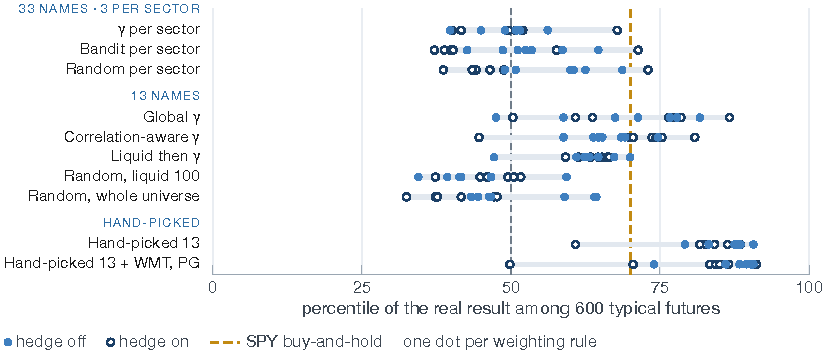
\includegraphics[width=\textwidth]{figs/supplement/figS_percentile.pdf}
    \caption{\textbf{Real-data results as percentiles of the typical synthetic futures.} For each selection rule and
    weighting rule, the percentile of the real terminal wealth ratio among the same cell's $600$ typical futures
    Filled dots have the market hedge off and open dots have it on (a $\beta$ cap that tightened as the market
    weakened, plus up to five names with $\beta \le 0$); the pale bar spans each row's lowest to highest dot. At $50$ (dashed) a real
    result equals the median future; the gold line marks real SPY, at the $70$th percentile of synthetic SPY. Real
    results use the seeds of the synthetic runs: the median over seeds $5660$--$5664$ for the random and bandit
    rules, and seed $5660$ for the rest.}
    \label{fig:S-percentile}
\end{figure}

% talk/data/b2_dots.csv, b2_bars.csv
\begin{figure}[H]
    \centering
    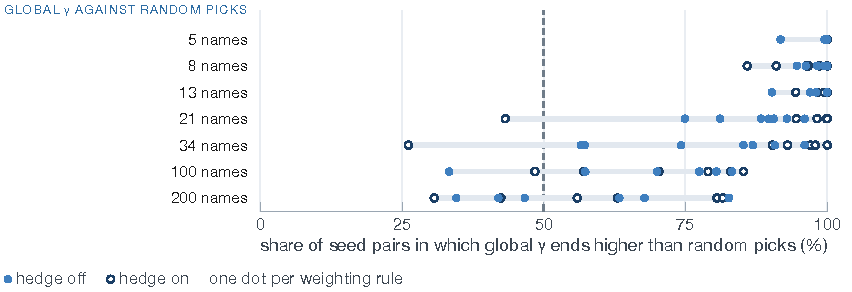
\includegraphics[width=0.9\textwidth]{figs/supplement/figS_size.pdf}
    \caption{\textbf{Global $\gamma$ against random picks from the whole universe, from $5$ to $200$ names, on real
    prices.} For each basket size and weighting rule, the share of the $900$ pairs of one global $\gamma$ run and one
    random run ($30$ runs each) in which global $\gamma$ ended with the higher terminal wealth ratio (market hedge
    off filled, on open). At $50\%$ (dashed) the two rules end higher equally often. Stone--Geary is left out at
    $100$ and $200$ names, where its baseline holding of $1\%$ of wealth per name uses the whole budget or twice the
    budget.}
    \label{fig:S-size}
\end{figure}
